\chapter{Experiments}
\label{experiments_chapter}
In this chapter, we will evaluate the performance of the various agents when
confronted with different combinations of obstacles, as well as presenting interesting observations made during the experiments. One of the key questions we aim to answer is whether any of the agents are a are capable of learning to play the entire game. To begin, it is important to explain how the experiments were conducted and the significance of the plots in the following subsections of this chapter.

\section{Conducting the experiments}
The process of conducting experiments encountered several challenges and fluctuations. Initially, the primary concern was to determine the appropriate number of rotations (\texttt{rots}) and distances (\texttt{dists}) for each obstacle type (explained in Table \ref{commOpt}). After experimenting with up to 30 rotations in some cases, and not getting satisfying results with seemingly any combination of other parameters, it was determined that the game's difficulty in later levels was the root of the problem, as it was impossible to play with some environments(confirmed by human players). Consequently, the game had to be adjusted and thus, there are slight variations in parameters, such as the starting speed and distances between obstacles, in the version of the ``Space-run'' game used in this thesis, as compared to the original. As per a human player's assessment, it is now possible to play all environment combinations until level 15 or even beyond. It is noteworthy that level 10 was the initial choice for the winning level, which was later shifted to level 15 to prevent the agent from settling for a mediocre policy and to find the optimal policy. However, this shift did not yield significant results, and the same behaviour could likely be achieved by increasing the number of games, allowing the $\epsilon$-greedy policy to perform random moves more frequently for an extended period. Despite this, level 15 was used in all subsequent experiments.

\begin{figure}[h]
    \centering
    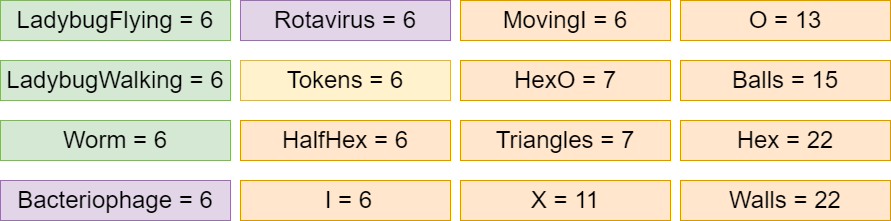
\includegraphics[width=0.8\textwidth]{rot_values}
    \caption{\texttt{rots} values used for each obstacle type}
    \label{fig:rot_values}
\end{figure}

After addressing the the issue of game not being playable, the most straightforward method for identifying the number of rotations required was to play the game manually in debug mode. The results obtained from these experiments are displayed in Figure \ref{fig:rot_values} and were used in all experiments conducted. However, for obstacles such as \texttt{Walls} and \texttt{Balls}, this method was not viable. The reason being that running \texttt{env=Balls} or \texttt{env=Walls} with visuals caused the game to lag significantly due to the number of animations playing simultaneously. As a result, \texttt{Walls} received the same number of rotations as \texttt{Hex} trap, while \texttt{Balls} received 15 rotations, the number at which the agent managed to learn. For bug, virus, and token obstacles, the default and minimum value of 6 rotations was assigned, with which they all trained successfully.
Concerning the \texttt{dists} parameter, it was concluded during the experiments that all agents could learn any obstacle with \texttt{dists=1}, and increasing this number needlessly would only increase the number of states required for training. 

The remaining values to be determined for the experiments were the suboptions for each agent (see \ref{opt:agent}).  The reader must realize that there were a lot of experiments conducted that had to be disregarded later on for this or that reason, but they provided useful insights that could be utilized. For instance, in many of those experiments, the agent performed best with \texttt{eps} values ranging from 0.2 to 0.4, with 0.2 being the most common, in combination with an \texttt{epsFinal} value of 0.0001. The rationale for using a low \texttt{epsFinal} value is that towards the end, the agent almost exclusively exploits the current policy, and a more gradual decrease in epsilon values is suitable for larger values of \texttt{n}. Furthermore, \texttt{initOptVal} of 20.0 and 100.0 was promising in most experiments. The \texttt{gam} value will be discussed in a later subsection.

Throughout the months dedicated to conducting experiments, they gradually converged towards checking combinations of the values mentioned above. In some instances, other values were experimented with and will be discussed when exploring various environments in later subsections. However, due to the length of the experiments and the number of parameters requiring adjustment, they were kept systematic towards the end, and most of the results presented in this chapter were obtained from experiments run with different \texttt{env} and value \texttt{n} adjusted according to the environment. Each combination was tested on ten seeds for each agent, with the combinations consisting of \texttt{eps} parameter taking a value of either 0.2 or 0.4, and the \texttt{initOptVal} being either 20.0 or 100.0. Discounting was kept at the value of 1 and \texttt{epsFinal} was 0.0001.

\section{Plotting}

\begin{figure}[h]
    \centering
    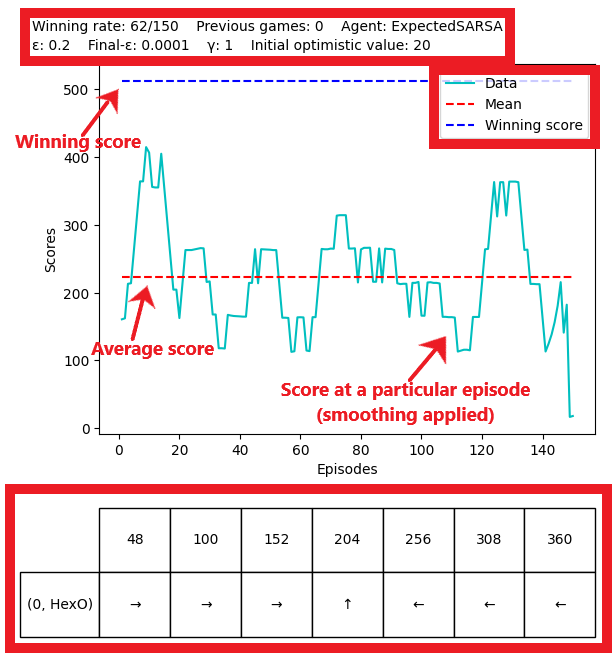
\includegraphics[width=\textwidth]{examplePlot}
    \caption{Plot example}
    \label{fig:plt_eg}
\end{figure}

In this chapter, a number of plots similar to the one shown in Figure \ref{fig:plt_eg} will be presented. This section has been dedicated to explaining the different components of these plots and how to read them. While some plots may differ slightly from the one in Figure \ref{fig:plt_eg}, the meaning behind them can still be easily deduced.

The top part of the figure displays all the necessary information that was used in the experiment. Most of the values have been previously described, except for ``Previous games''. This value is meant for experiments that used the \texttt{database=read} option and were performed on an agent that had trained for some number of games. This number specifies the how many of games the agent had previously trained on.

Moving further down, there is a plot with three lines and a legend in the top right corner. The data line, as indicated on the figure, represents the score that the agent achieved on a particular episode. However, some plots may show the average value of the agent's score for that episode over several different seeds used for the random action. Additionally, there may be multiple data lines on the plot, each averaged between many seeds and each representing a different agent. Every agent is labelled with their respective color inside the legend.

The mean line represents the average score value for the entire experiment, while the winning score represents the winning threshold which is the score that the agent achieves after passing level 15. This score will be constant, except in the cases where the environments contains any of the bugs and viruses and the agent is allowed to shoot. The winning score then depends on how many of those obstacles the agent successfully shoots. In this case the line will show the winning score of the last game in which the agent won. It should be noted that if the agent did not win any games, or the plot is displaying multiple agents, the winning score line will be omitted. Furthermore, the data line is averaged to appear smoother. This is why even though the winning rate is 62/150 in this sample plot, the data line doesn't touch the winning score threshold at any point.

As mentioned in Section \ref{commOpt}, it is possible to perform continuous evaluation on experiments, meaning one learning game is played with random actions, followed immediately by an evaluation game using only the current policy that the agent is performing. In all experiments conducted, the data line only represents the evaluation games.

At the very bottom of the figure, there is a table which only appears in plots that contain a single data line that is not averaged over different seeds and has only one seed value. In the table, all rotation values for this experiment define the columns, while each row has a tuple of distance value and type of the obstacle. Each cell then represents a particular discrete state, and the arrow it shows is the action that the agent takes in that state. If the arrow has \textit{*} attached to it, it means that the agent will also shoot. Since all experiments are performed on \texttt{dists=1}, the number of rows will match only the number of different obstacles used in the experiment.

It should be emphasized that parameters such as the number of seeds in the averaged data line or the size of the smoothing window will be clearly specified for each plot mentioned in the rest of the chapter. This prevents any form of ambiguity or confusion regarding the details of the experiment.

\section{Interesting behaviours}
\label{intbeh}
\begin{figure}[h]
    \centering
    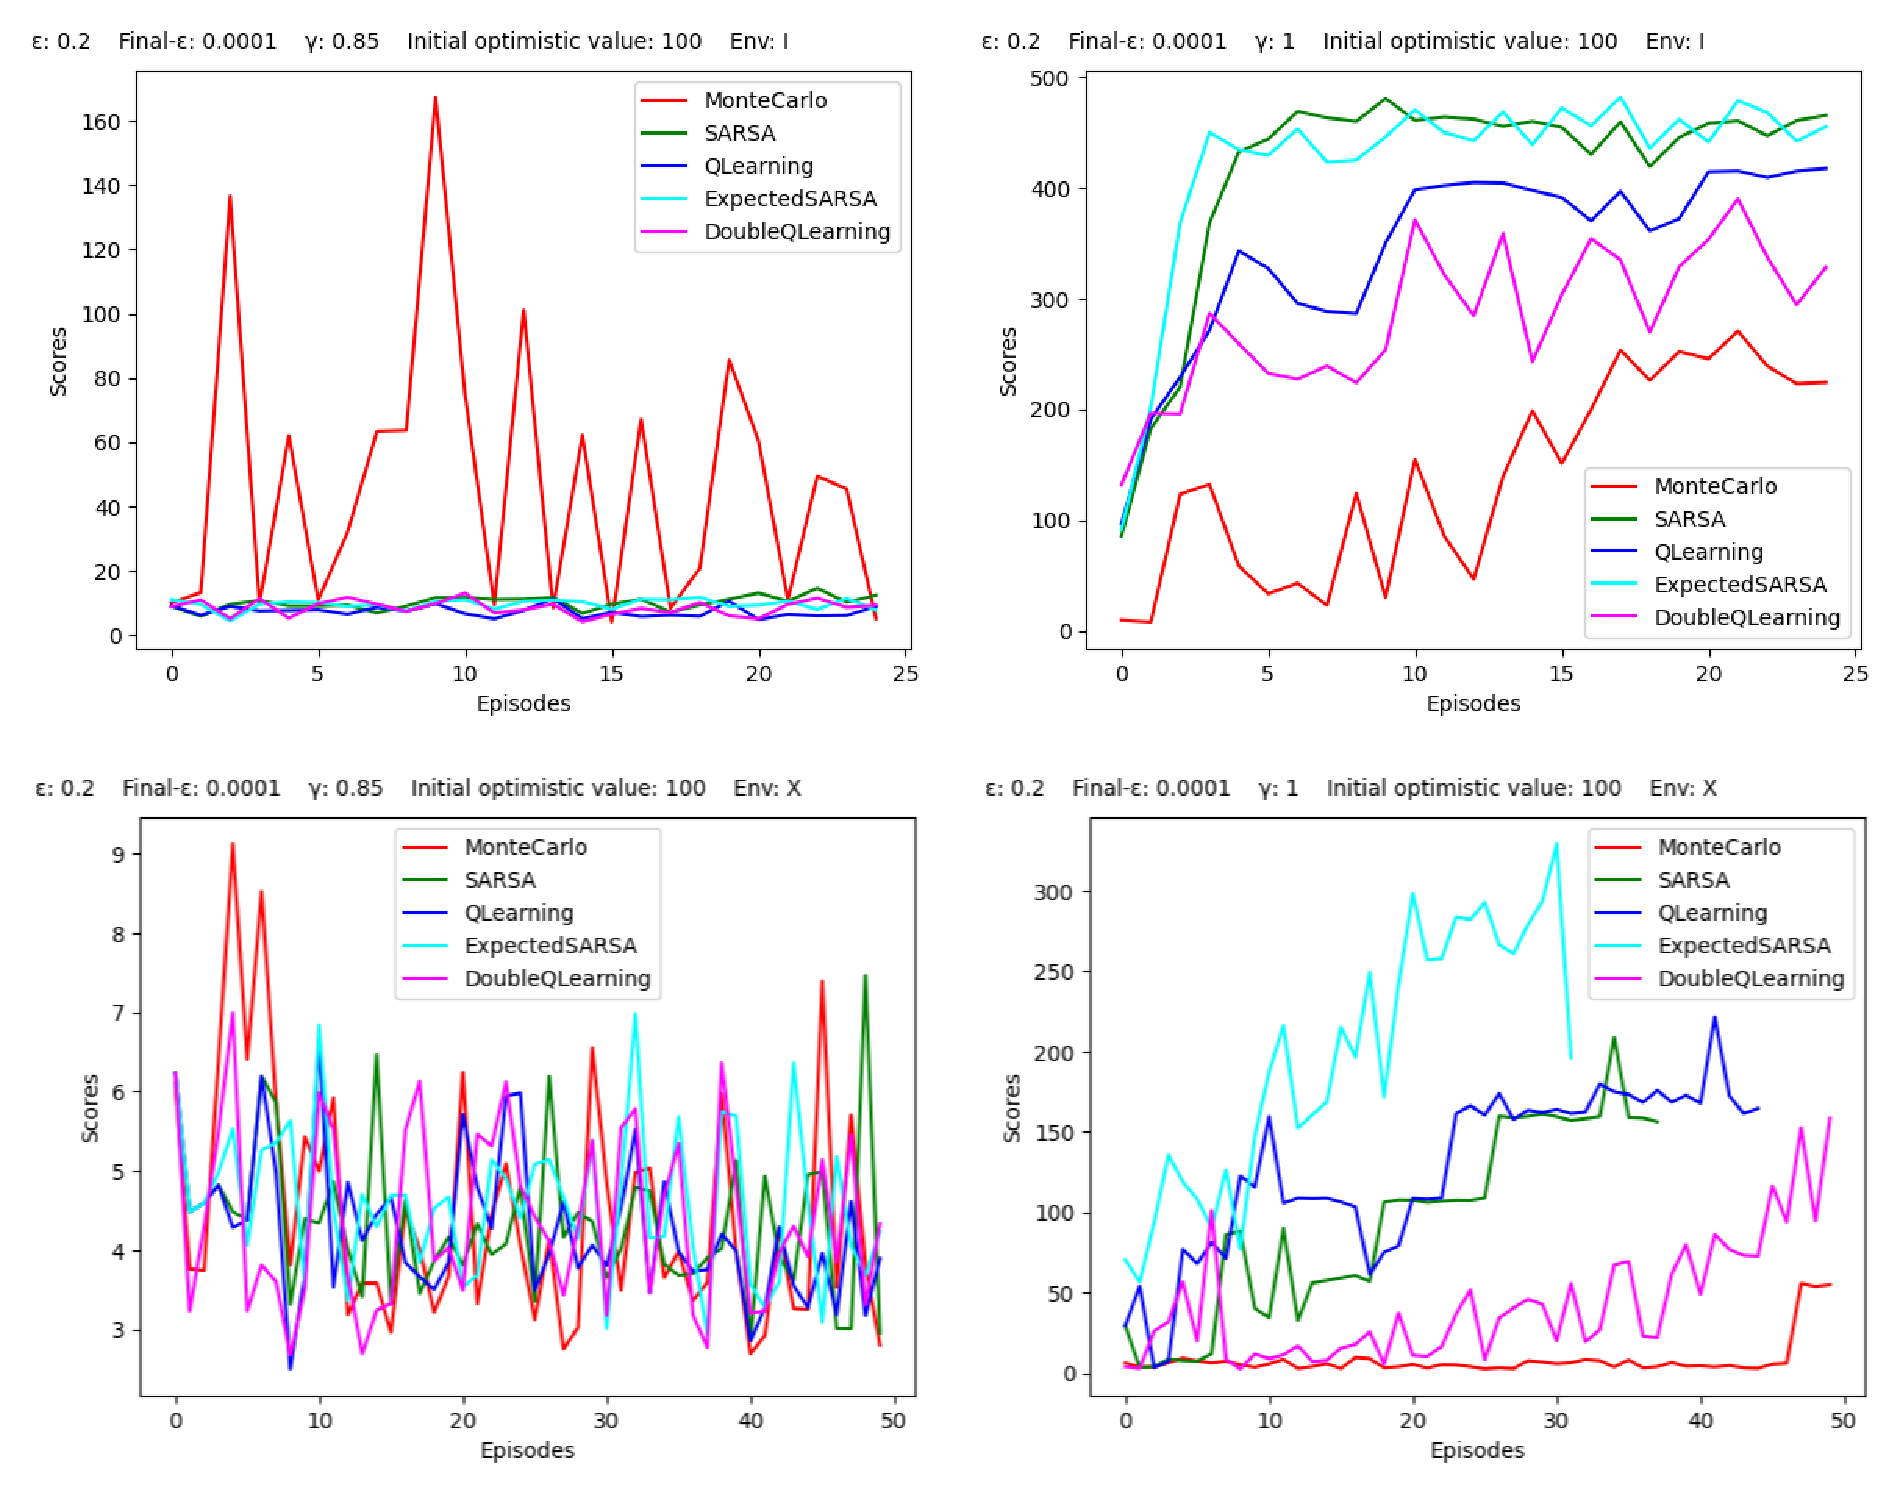
\includegraphics[width=\textwidth]{discountingExample}
    \caption{Discounting example}
    \label{fig:discounting_eg}
\end{figure}

In this chapter, we aim to discuss certain unexpected findings that surfaced during our experimentation. One of the immediate observations can be seen in Figure \ref{fig:discounting_eg}\footnote{No smoothing was applied to any of the plots in this subsection.}. We conducted experiments on two distinct environments, \texttt{env=[I]} and \texttt{env=[X]}, and for each environment, we carried out experiments with discount rates of \texttt{gam=0.85} and \texttt{gam=1.0} for all agents. As evident from the plots, the lower gamma value exhibited considerably poorer performance than when no discounting (\texttt{gam=1.0}) was applied. This trend is not limited to these specific environments and testing conditions but rather observed consistently across all our experimentation. This result is counter-intuitive since it seems logical that penalizing the last action more than previous ones would result in a better policy.

\label{intbeh}
\begin{figure}[h]
    \centering
    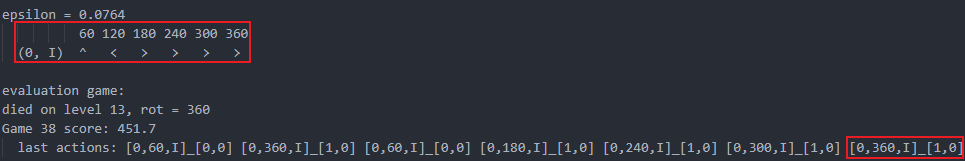
\includegraphics[width=\textwidth]{discountingExplanation}
    \caption{Discounting explanation}
    \label{fig:discounting_expl}
\end{figure}

Upon further investigation, we discovered that in some cases, a lost game for the agent does not result from the last action directly but rather from a chain reaction initiated by a previous bad decision. As seen in Figure \ref{fig:discounting_expl}, the agent's last action of going right at rotation \texttt{360} to reach a safe one, \texttt{60}, is not a poor decision in itself but rather the best possible action in that state\footnote{As confirmed by a human player, rotation 60 is safe for trap type I.}. However, analysing the last four actions taken by the agent, it becomes clear that it attempted to reach rotation \texttt{60} by going left from the rotation \texttt{180}. With a high score of \texttt{451.7} (Figure \ref{fig:discounting_eg}), the agent undeniably had high speed value, making it move forward very quickly, and while this policy may have been effective in the early game before the agent attained its current speed\footnote{It should recalled that after every 3 levels the agents speed increases.}, there is simply not enough time for the agent to rotate at this point in the game. In this case, one could argue that the fourth action from the last was responsible for the agent's loss. For cases like this, we believe that the agent performs better when all actions are penalized equally.


\label{intbeh}
\begin{figure}[h]
    \centering
    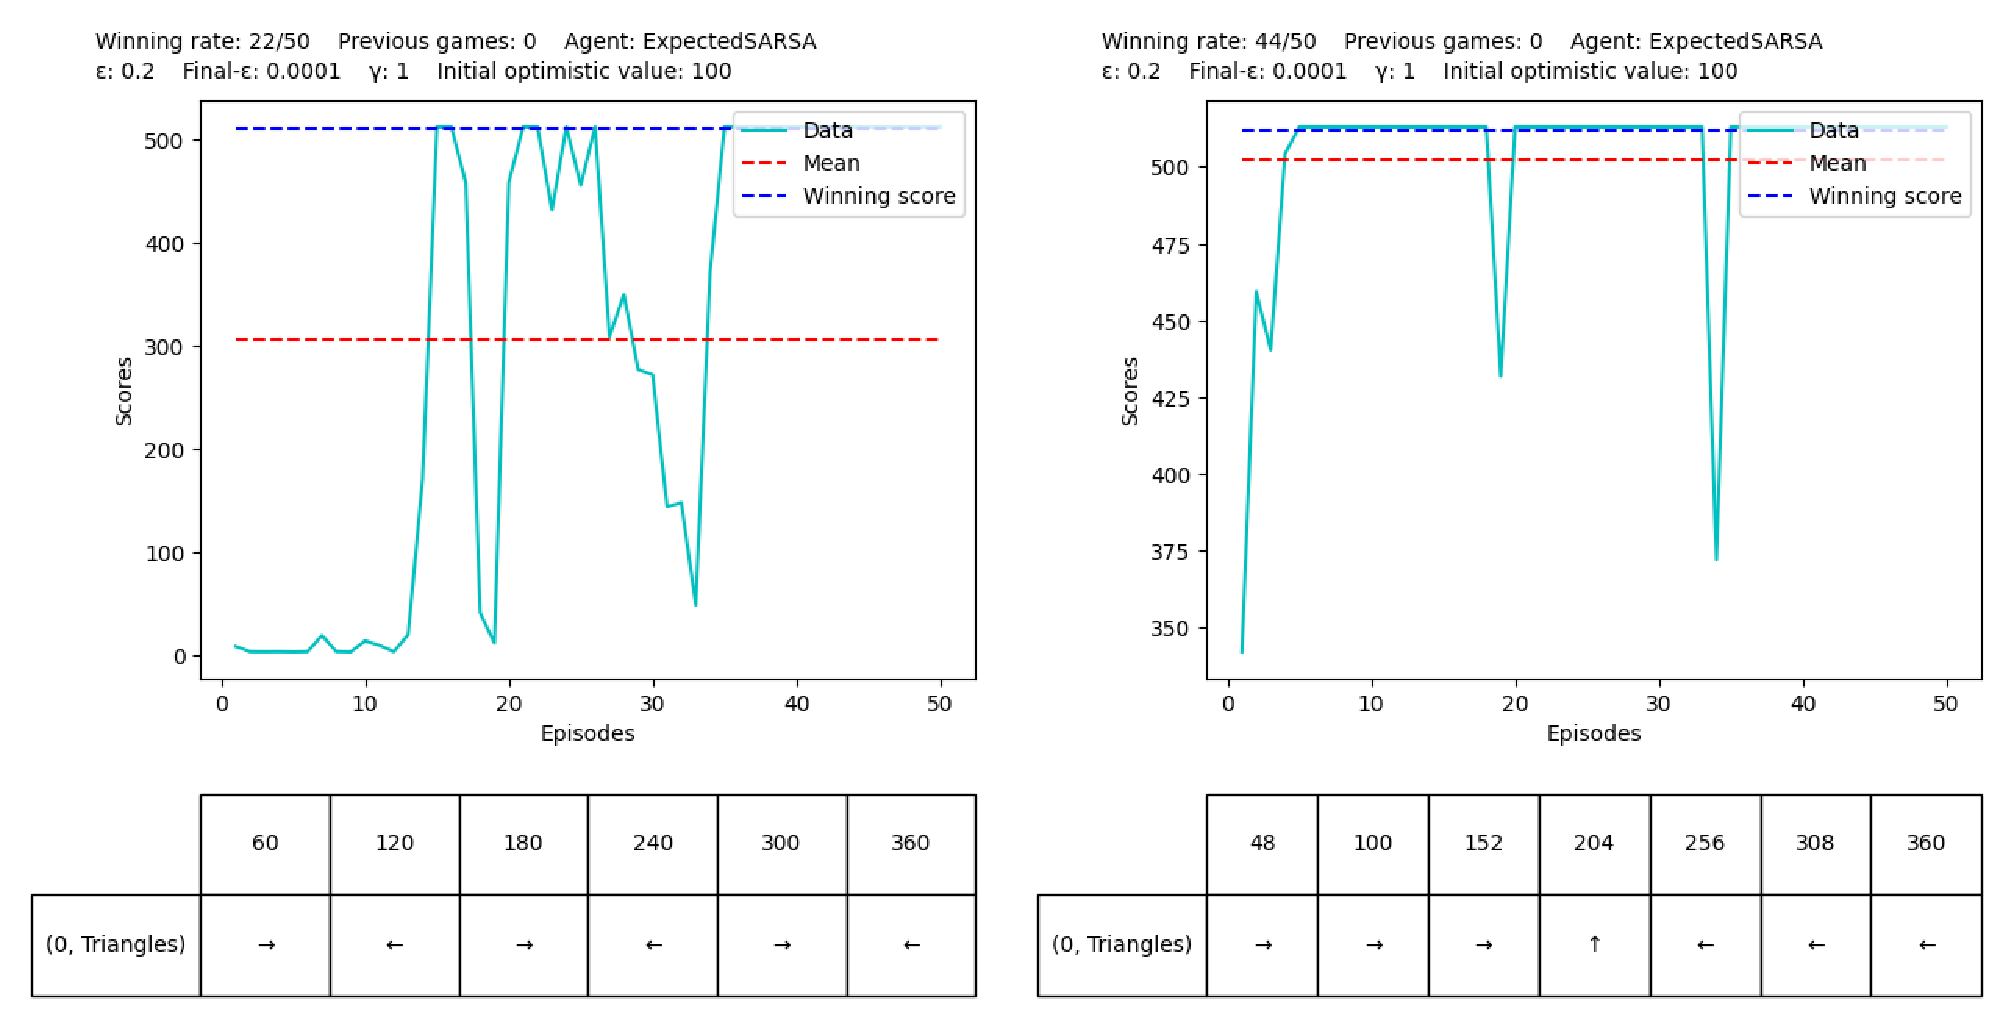
\includegraphics[width=\textwidth]{trianglesExample}
    \caption{\texttt{Triangles} example}
    \label{fig:triangles_intbeh_eg}
\end{figure}

Another intriguing behaviour emerged as a result of our learning architecture. As previously noted, we chose to have the agent not take a new action every time its \texttt{move()} function is called, but rather return the same action until the state changes. This resulted in a substantial reduction in the number of different actions taken by the agent, given that the move function is invoked every game tick, while state changes occur less frequently. This approach led to a behaviour that could not have been predicted at the outset. Figure \ref{fig:triangles_intbeh_eg} provides an illustration of this behaviour (with some sentiment \texttt{env=[Triangles]} was chosen as this was the first environment on which the behaviour was noticed).

Ordinarily, \texttt{env=[Triangles]} does not offer any safe rotations unless \texttt{rots=7} or more. As shown in the plot, the agent will certainly learn with this rotation value. However, if the agent is given only \texttt{6} rotation values to choose from, it will develop a policy that rapidly oscillates between two rotations, keeping the player character, Hans, on the edge of those rotations, allowing him to safely pass through the trap. This behaviour is not confined to situations where the agent is ``forced'' to make such a decision. During training, in many instances, the agent will learn to stay on the edge rather than advance into a completely safe rotation. There does not appear to be a preference for one or the other; rather, the policy the agent discovers first is determined by other experimental factors. It can be concluded that this behaviour arose solely because the agent did not alter its action until the state changed. In my opinion, this discovery is one of the most exciting outcomes of this project.

\section{Individual traps environments}
This section discusses the performance of agents in environments containing only one trap at a time.  Considering the number of traps and agents, for each trap, we have picked a plot that showed the best performances of the agents overall. Some specific cases will, of course, be highlighted. It should be noted that all plots within these examples have had smoothing applied with \texttt{window=10}. Thus certain spikes will not be visible. Additionally, unless otherwise suggested, you can assume that the values that were produced are an average of 5 different seeds. The aim was to show a realistic picture on how the agent would perform, and not show the occurrences in which the outcome was satisfactory but rather account for the failures in reproducing the perfect policy as well.

\begin{figure}[h]
    \centering
    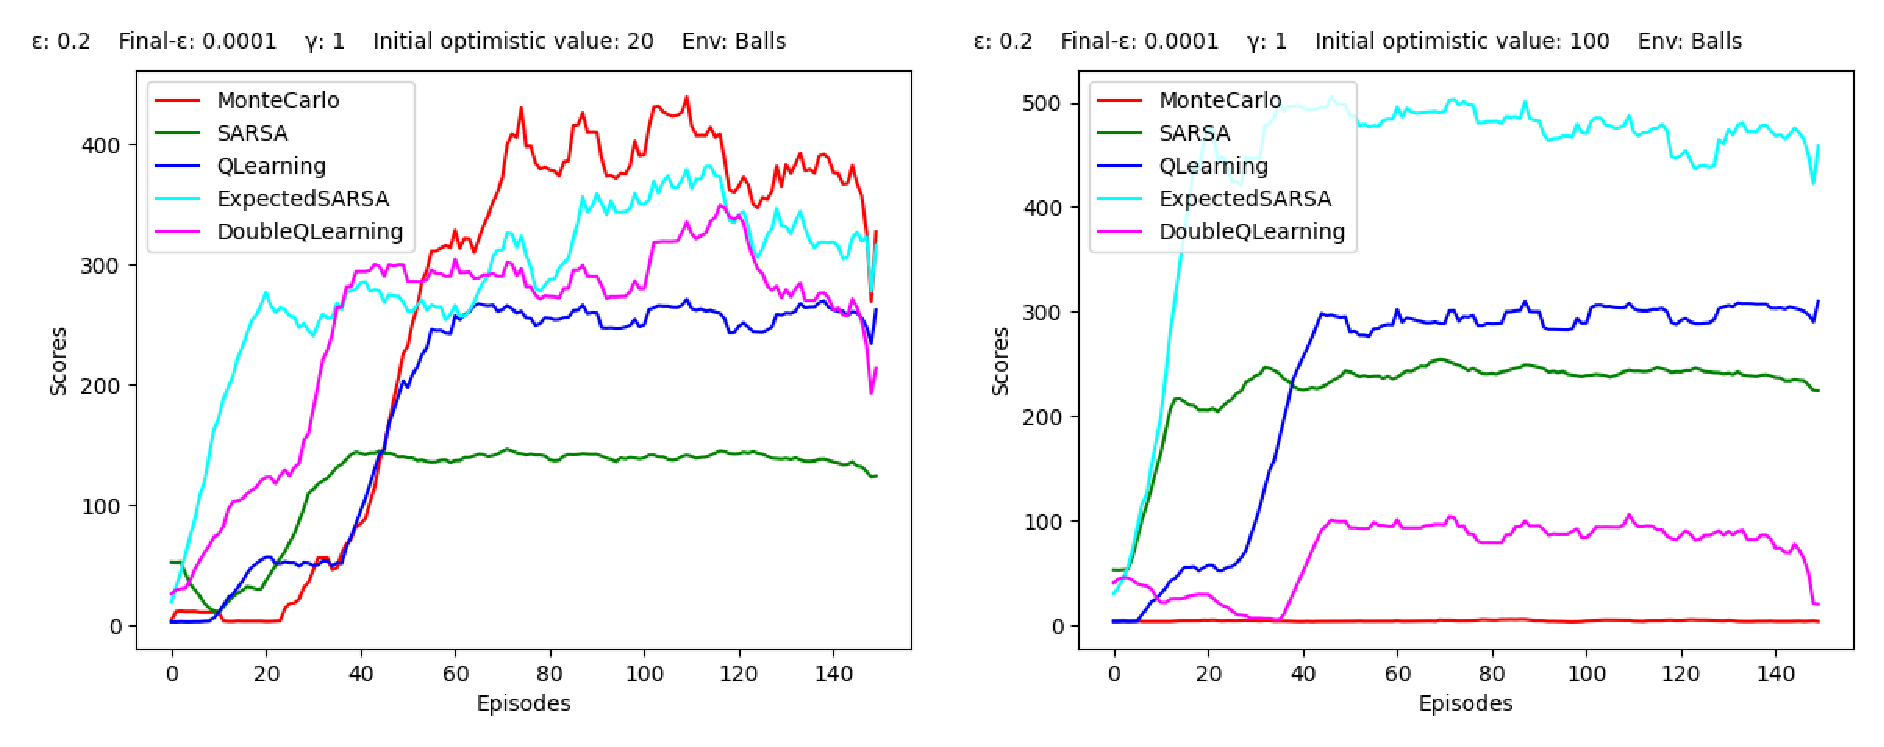
\includegraphics[width=\textwidth]{balls}
    \caption{\texttt{Balls} trap examples}
    \label{fig:balls_eg}
\end{figure}

\begin{figure}[h]
    \centering
    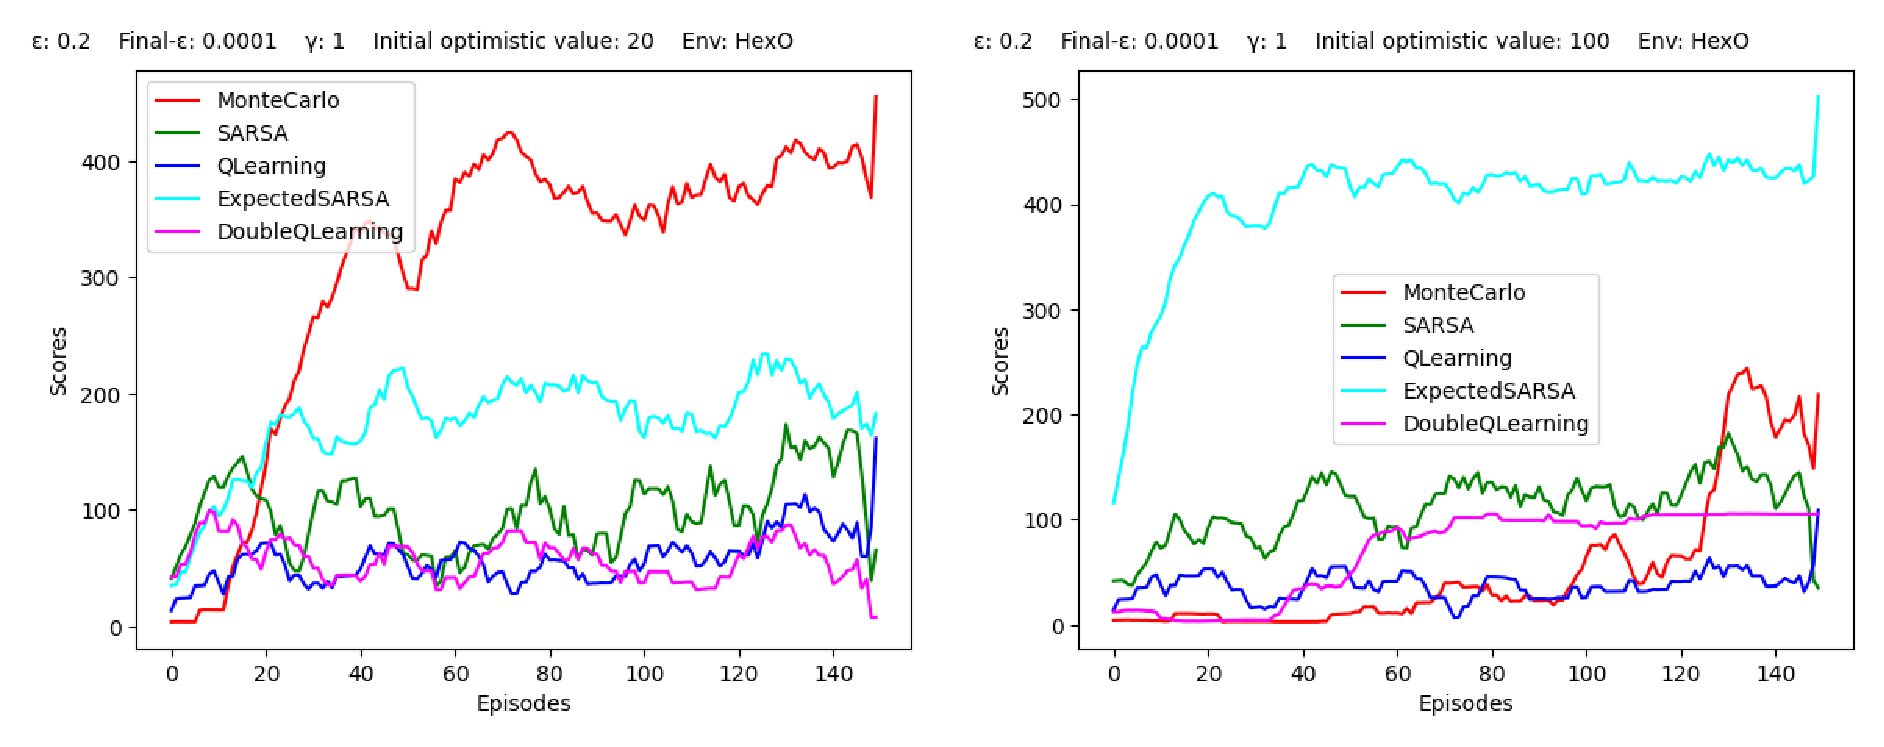
\includegraphics[width=\textwidth]{hexo}
    \caption{\texttt{HexO} trap examples}
    \label{fig:hexo_eg}
\end{figure}

Another very important factor were the choices of the hyperparameters. As mentioned before, most the commonly values will be \texttt{eps=0.2} or \texttt{eps=0.4} and \texttt{initOptVal=20.0} or \texttt{initOptVal=100.0}. Perhaps best visible in Figures \ref{fig:balls_eg} and \ref{fig:hexo_eg}, is how much hyperparameters can influence the outcome. Both the \texttt{Balls} and \texttt{HexO} traps varied significantly based on the initial optimistic value used, with the other agents' performances also varying to a lesser extent. These findings underscore the importance of carefully selecting hyperparameters when training reinforcement learning.

Nevertheless, in some cases we have not managed to find the right combination of the hyperparameters. The Hex trap is a prime example of such a challenge, requiring no less than 22 rotations to be navigated successfully. As shown in Figure \ref{fig:hex_eg}, the agents' overall performance on this trap has been moderate at best.

\begin{figure}[h]
    \centering
    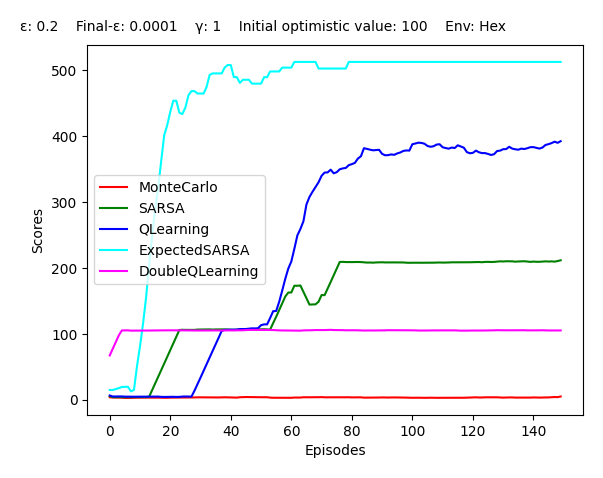
\includegraphics[width=0.7\textwidth]{hex}
    \caption{\texttt{Hex} trap example}
    \label{fig:hex_eg}
\end{figure}

\begin{figure}[h]
    \centering
    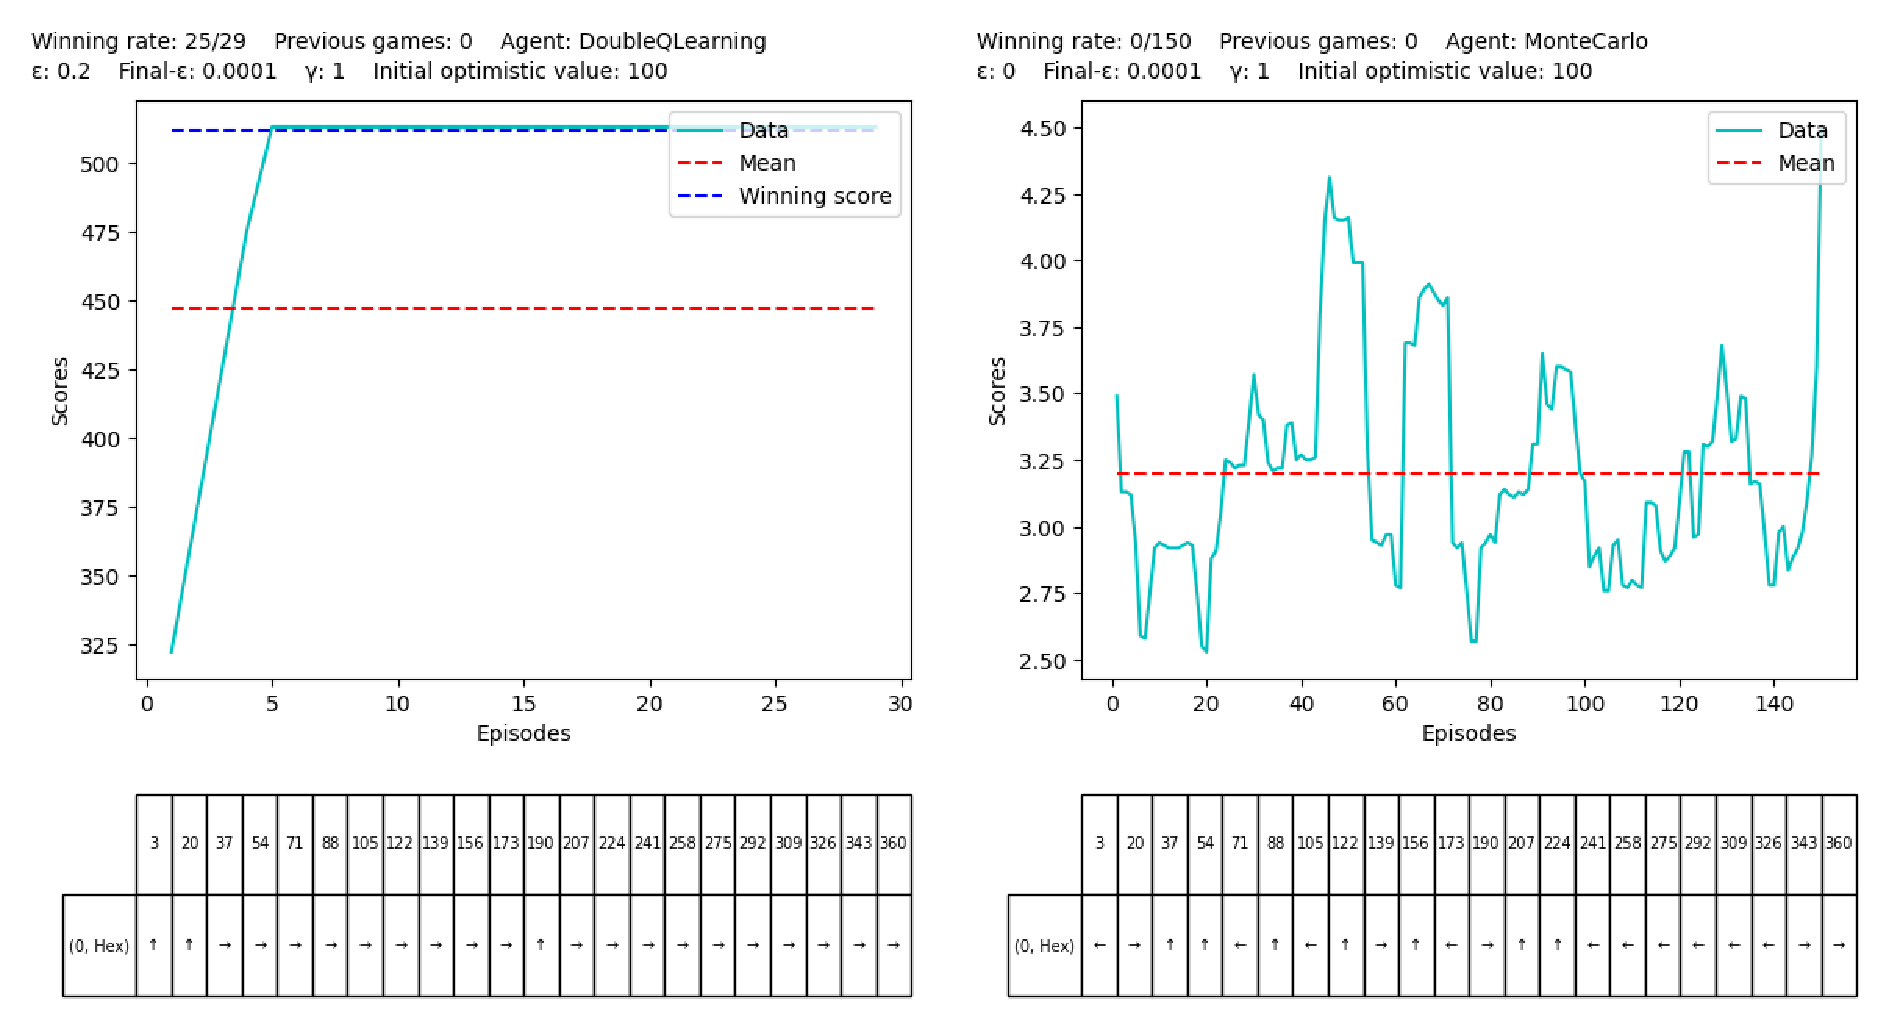
\includegraphics[width=\textwidth]{hex_dql_mc}
    \caption{\texttt{Hex} trap with \texttt{DoubleQLearning} and \texttt{MonteCarlo} agents}
    \label{fig:hex_diff_eg}
\end{figure}

However, Figure \ref{fig:hex_diff_eg} presents the results of an experiment conducted on the \texttt{MonteCarlo} agent, which was produced by a single seed value. The choice of seed or hyper parameter values is not critical, as all the values for the Hex trap for this particular agent lead to similar performance. By examining the policy that the \texttt{MonteCarlo} agent learned in this experiment and comparing it to the left-hand plot, which depicts the \texttt{DoubleQLearning} agent learning an arguably perfect policy right from the start, we can see that the \texttt{MonteCarlo} agent completely overlooks the safe rotations and instead chooses to move forward in areas that lead to either certain death, or half-safe rotations which let the agent pass based on pure chance. It is worth noting that the performance of the \texttt{DoubleQLearning} agent varies depending on the seed value (on the plot in Figure \ref{fig:hexo_eg} we can see that the average performance of \texttt{DoubleQLearning} agent is actually lower than for the other agents, excluding \texttt{MonteCarlo}), and this example was included only to illustrate what an optimal policy for this type of trap might look like.

\begin{figure}[h]
    \centering
    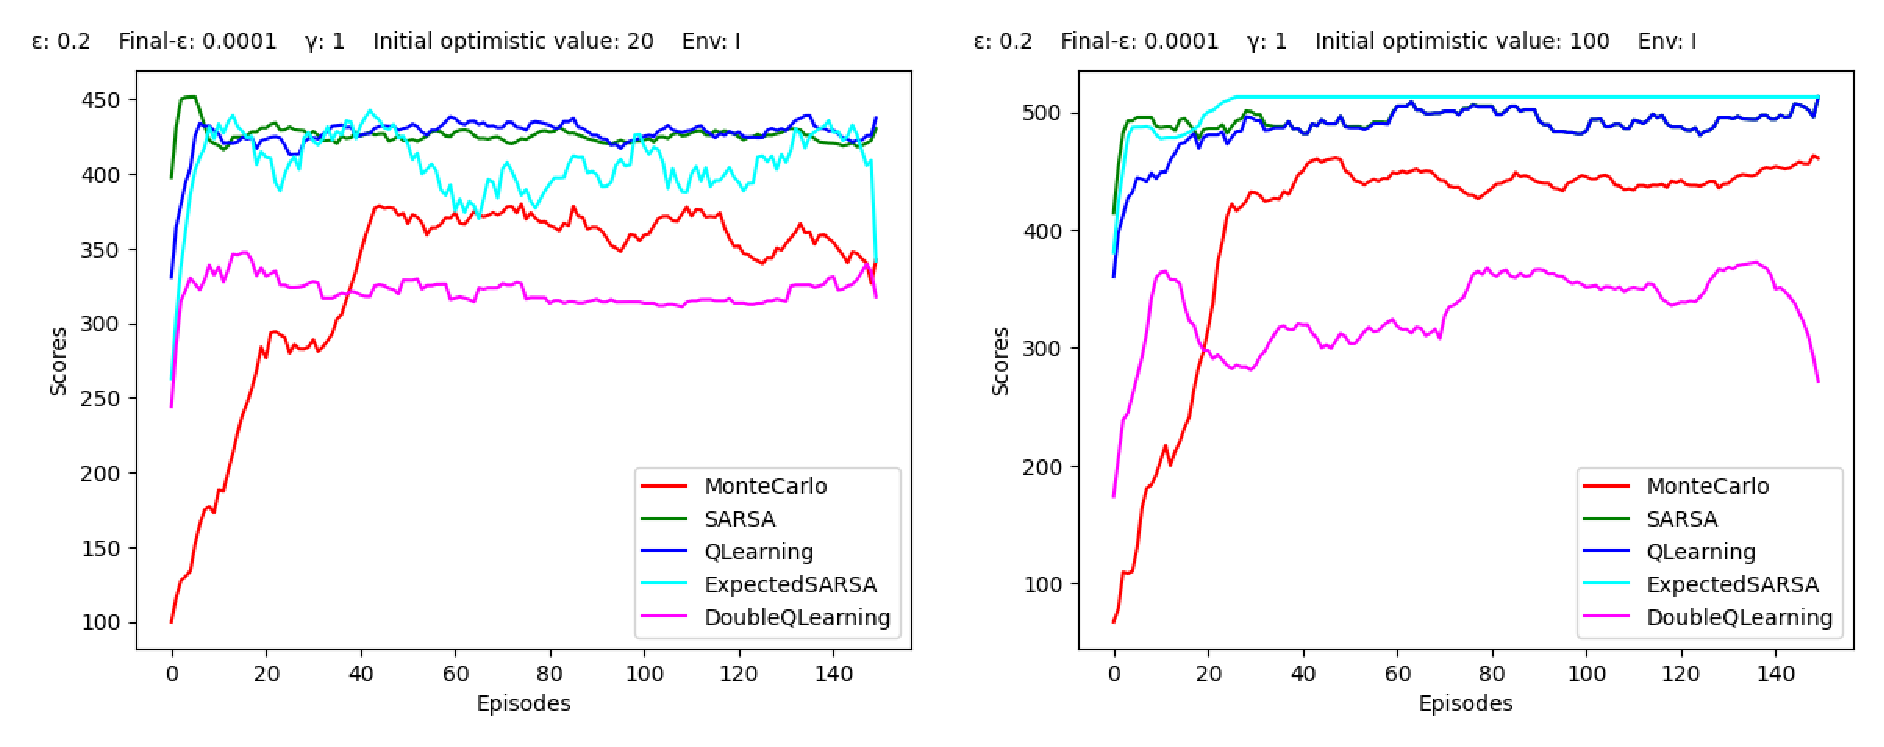
\includegraphics[width=\textwidth]{i}
    \caption{\texttt{I} trap examples}
    \label{fig:i_eg}
\end{figure}

\begin{figure}[h]
    \centering
    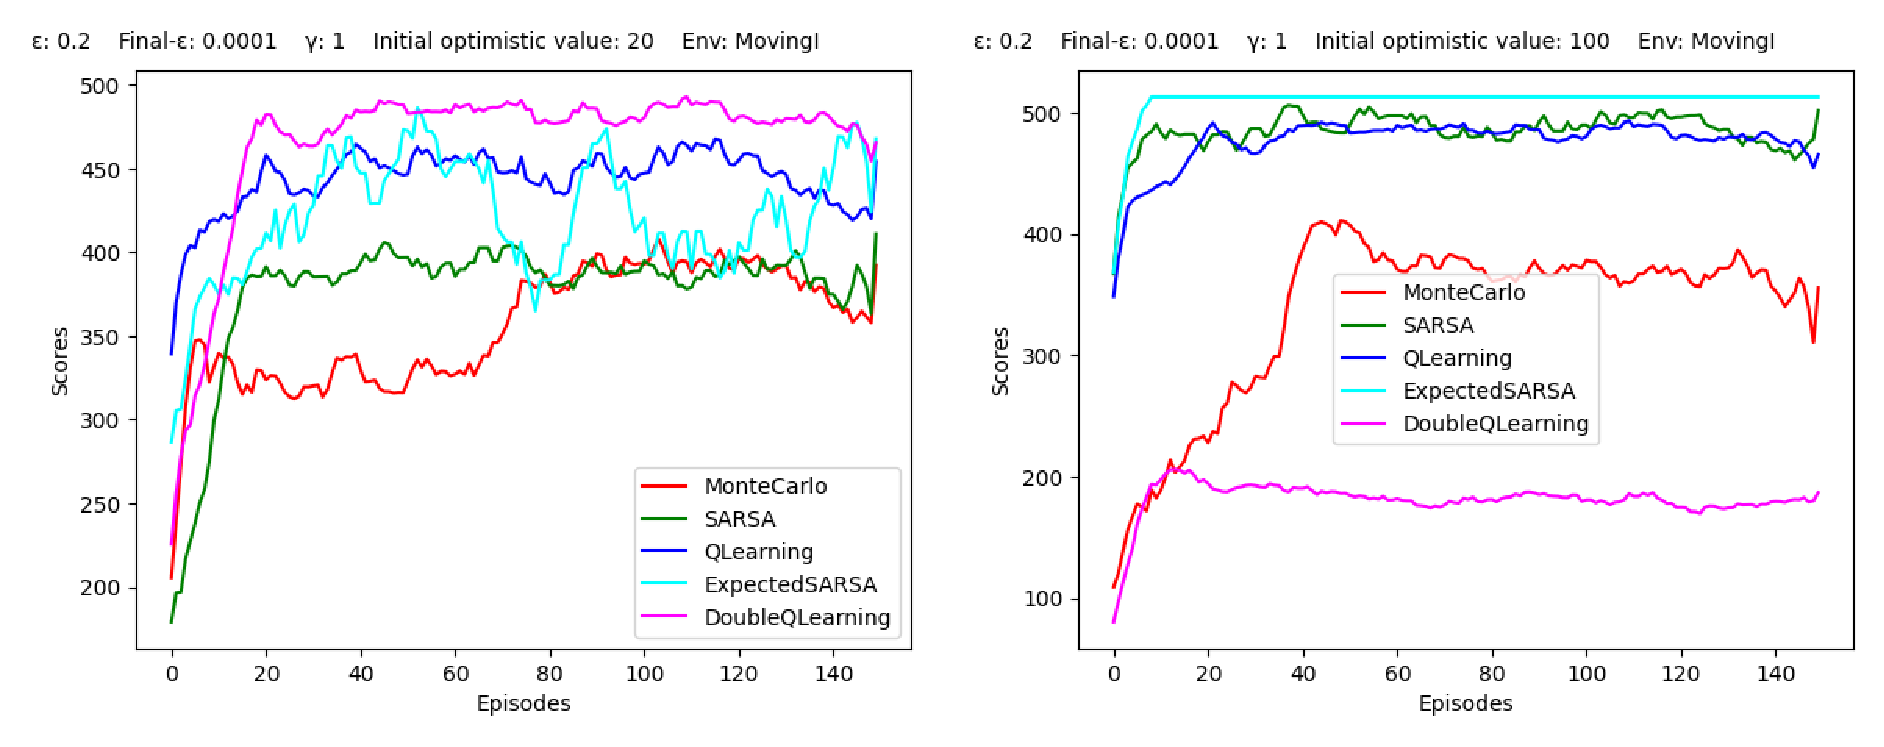
\includegraphics[width=\textwidth]{movingi}
    \caption{\texttt{MovingI} trap examples}
    \label{fig:movingi_eg}
\end{figure}


It is worth noting that there exist cases where the aforementioned variations in hyper parameter selection lead to highly desirable outcomes. This is exemplified by the results presented in Figures \ref{fig:i_eg} and \ref{fig:movingi_eg}, which demonstrate the efficacy of the \texttt{ExpectedSARSA} agent. Notably, on the right hand side of the both plots, the \texttt{ExpectedSARSA} agent was able to achieve optimal performance early on in the game with all seed values. \texttt{ExpectedSARSA} agent, in a very large number of experiments, has outperformed its counterparts, sometimes by a significant amount. This is particularly evident when considering its performance in simpler environments such as traps \texttt{I} and \texttt{MovingI}, where it is apparent that the agent is capable of learning extremely well. While other agents have performed well on these specific traps as well, their success may not be immediately apparent from the averaged results depicted in the plots.

As can be observed from some of the previous graphs, agents often exhibit significant changes in behaviour with different hyperparameters. However, as depicted in Figure \ref{fig:triangles_eg} for the \texttt{Triangles} trap, increasing the \texttt{initOptVal} resulted in the agents maintaining the same ratio between each other, despite three of them increasing their average score significantly.

\begin{figure}[h]
    \centering
    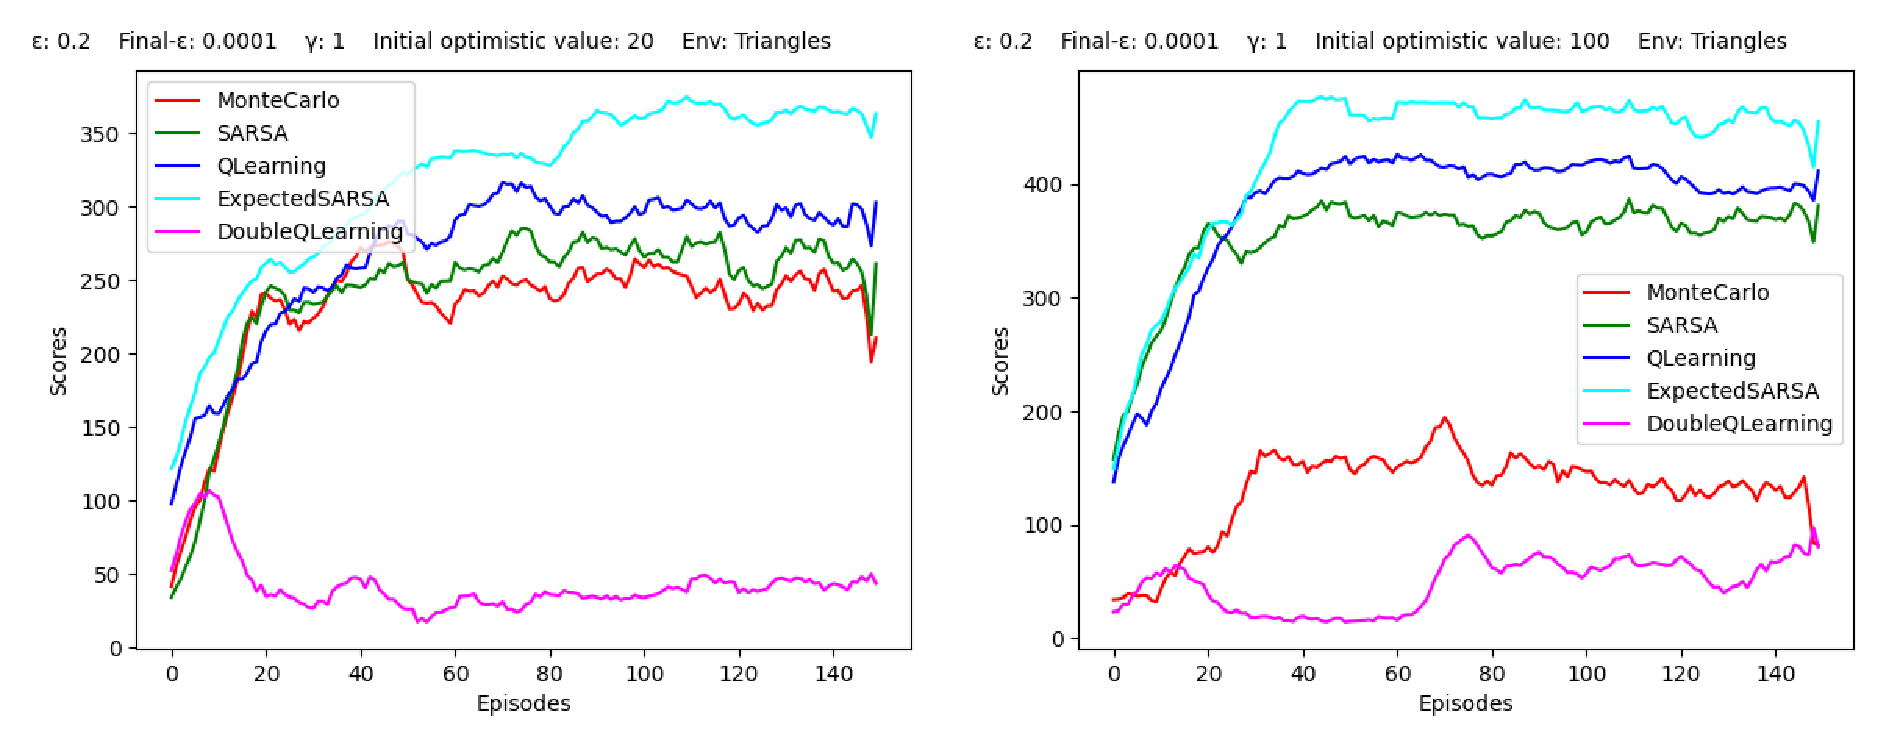
\includegraphics[width=\textwidth]{triangles}
    \caption{\texttt{Triangles} trap examples}
    \label{fig:triangles_eg}
\end{figure}

\begin{figure}[h]
    \centering
    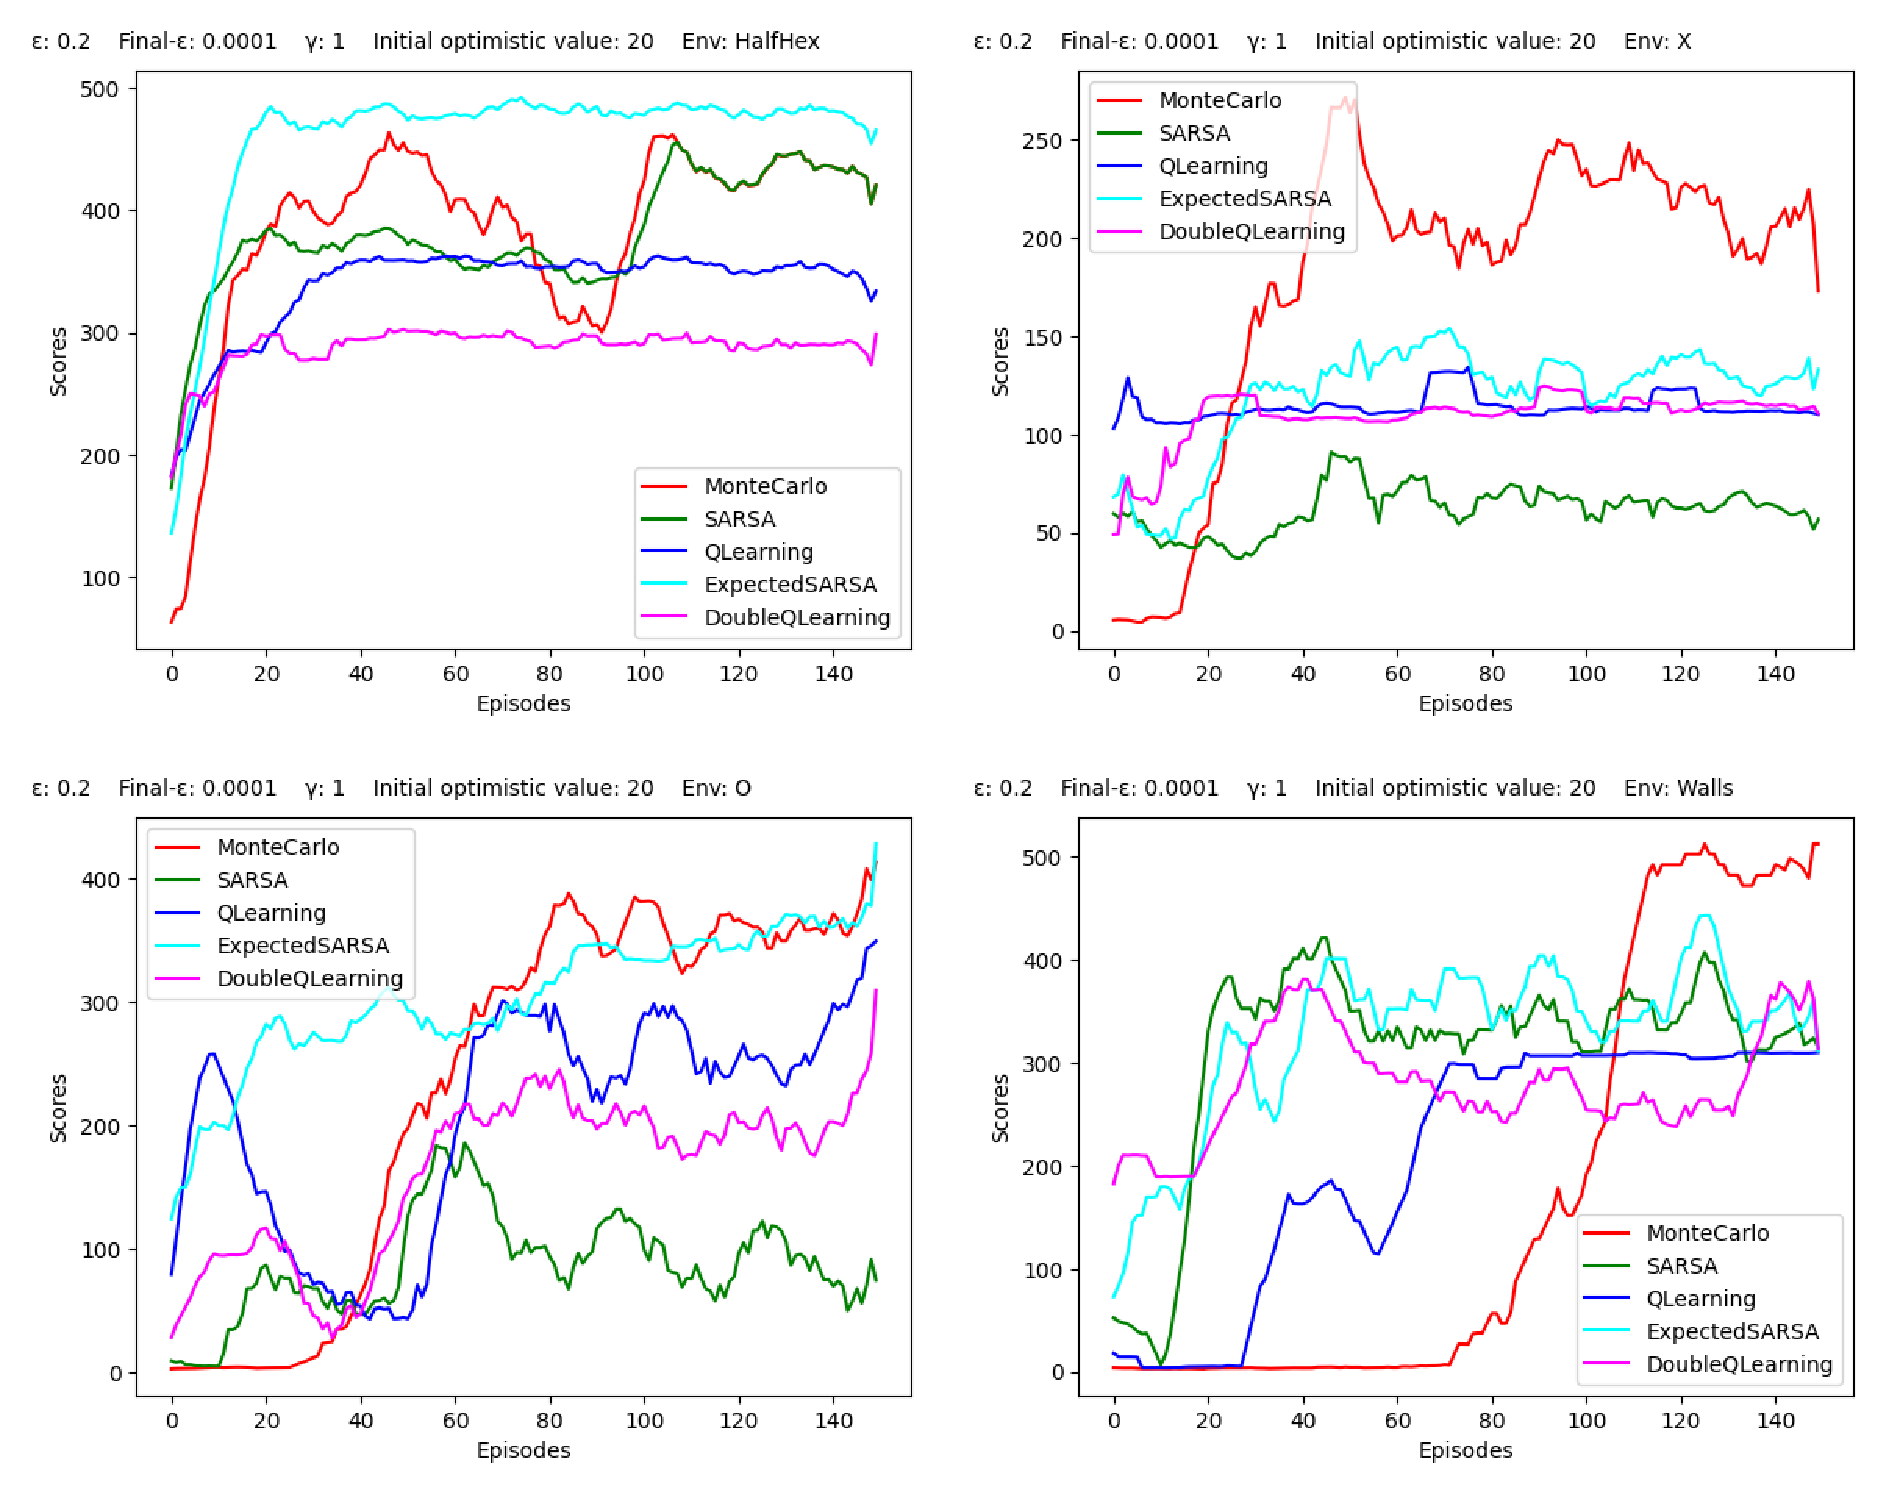
\includegraphics[width=\textwidth]{halfhex_o_walls_x}
    \caption{\texttt{HalfHex, X, O} and \texttt{Walls} traps examples}
    \label{fig:halfhex_o_walls_x_eg}
\end{figure}

Figure \ref{fig:halfhex_o_walls_x_eg} showcases the performance of the agents on the remaining traps that have not been mentioned before in this section. It is worth noting that the agents' overall behaviour on these traps is satisfactory, with some agents performing exceedingly well. This, once again, reinforces the idea that the choice of hyperparameters can have a significant impact on the agent's performance, and that a careful selection of these parameters is crucial for achieving optimal results.

Although performing these experiments with a larger number of seeds would ideally yield even more accurate results, we hope that the picture we presented provides a reasonable representation of the agents' performance.

\section{Traps environment}
\begin{figure}[h]
    \centering
    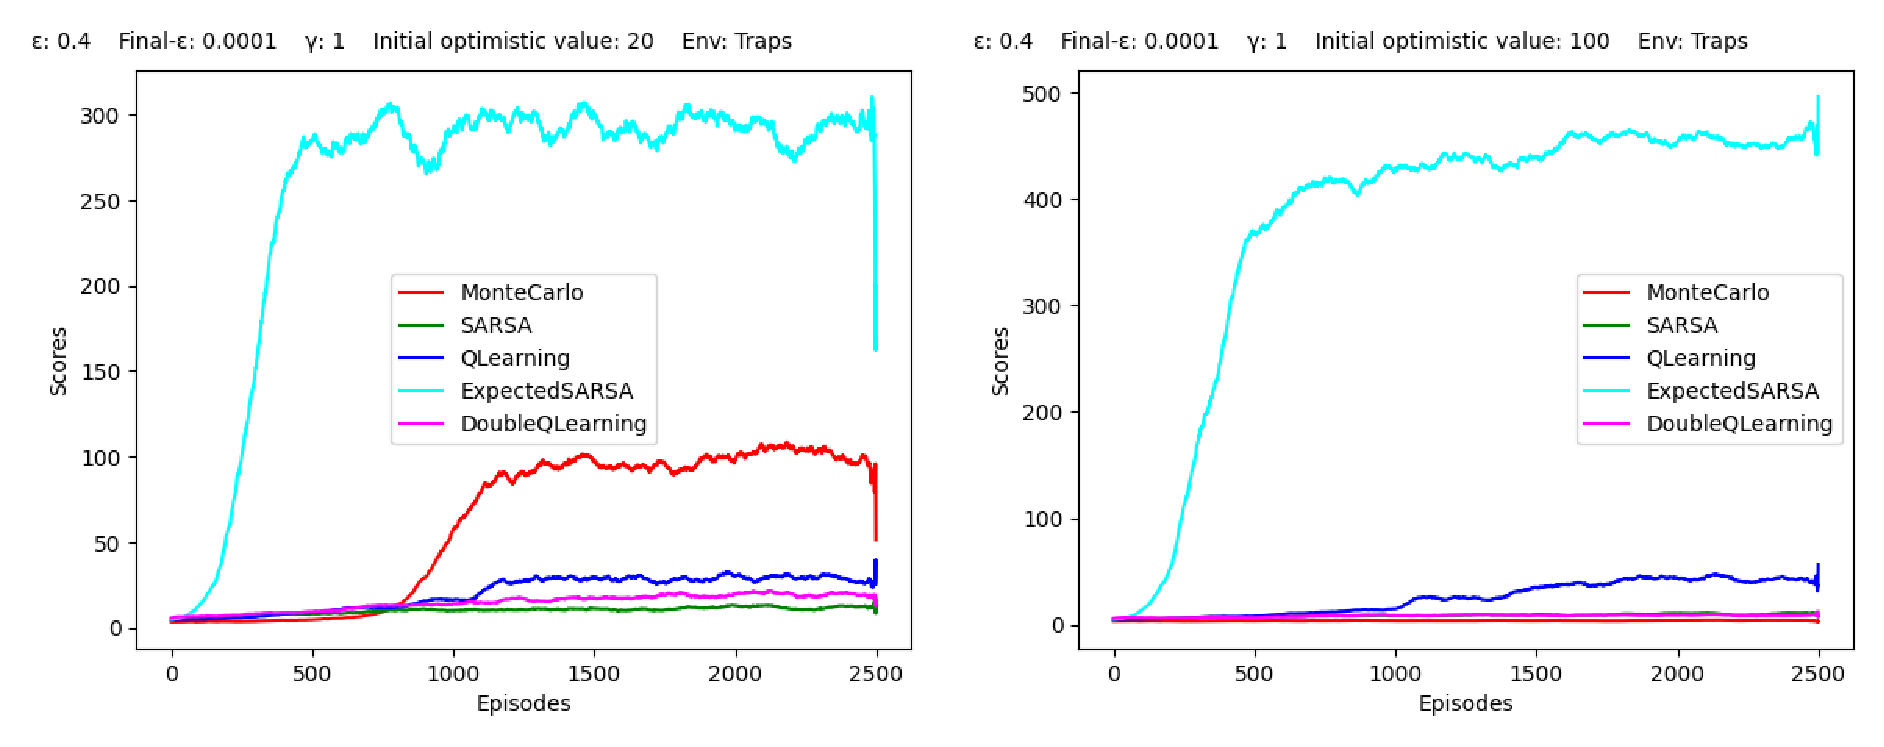
\includegraphics[width=\textwidth]{allTraps}
    \caption{All traps examples}
    \label{fig:alltraps_eg}
\end{figure}

This section delves into the exploration of a highly intricate environment of all traps combined, which is possibly the most complex one barring the full game. To clarify,\trexttt{Traps} consist of all 10 individual traps mentioned in the previous section, and omit any bugs, virus or token type of obstacles. As depicted in Figure \ref{fig:alltraps_eg}, the majority of agents were unable to perform optimally in this environment. \texttt{ExpectedSARSA} was the only agent able to learn an optimal policy in any occurrence, as evidenced by its score nearing 500 in the right plot\footnote{It is worth mentioning that the plots for this environment have been smoothed with \texttt{window=100}.}, which was the approximate winning score value in all experiments. Moreover, \texttt{ExpectedSARSA} not only managed to learn an optimal policy once but did so with different hyperparameters and seed values on multiple occasions, leading to winning streaks of 30 games and early termination of the experiment. This outcome is the most favourable for any environment. The figure displays the averaged value of 9 seeds for all agents under the specified parameters. 

The experiments conducted for this environment were systematic and involved matching commonly used \texttt{eps} and \texttt{initOptVal} to test if the agents could learn. In these experiments, the difference in learning between the \texttt{ExpectedSARSA} agent and the others is even more pronounced. However, on the left plot visible in Figure \ref{fig:alltraps_eg}, and one instance, where \texttt{eps=0.4} and \texttt{initOptVal=20}, the \texttt{MonteCarlo} agent performed reasonably well, attaining an average score of approximately 100, which is substantially superior to the other agents, except for \texttt{ExpectedSARSA}.

\begin{figure}[h]
    \centering
    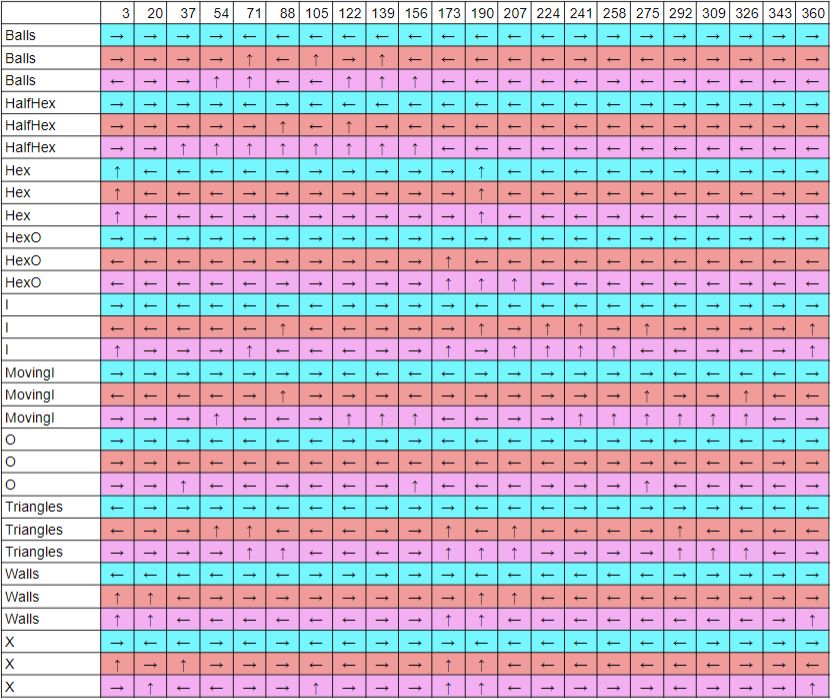
\includegraphics[width=\textwidth]{allTraps_table}
    \caption{All traps with \texttt{ExpectedSARSA}, \texttt{MonteCarlo} and \texttt{DoubleQLearning} agents}
    \label{fig:traps_table_eg}
\end{figure}

When training in the all-traps environment I set the rots parameter to 22.  That's because it contains the Hex and Walls traps, which require a minimum of 22 rotations for learning to be feasible at all. This means that the number of states that with the individual trap environments corresponded to number of rotations, increased significantly. Considering that in this case we have 10 different trap types, there are 220 states with \texttt{Traps} environment. For that reason we picked \texttt{n=2500} for all of the experiments in this section. That's because in our experiments we've generally found that learning is most successful when the number of episodes is at least 10 times the number of states. Of course, it cannot be influenced by which states will be picked, since each game is generated randomly, but this was an estimation we used quite often during the experimentations. As a result of having this many \texttt{rots} values, with some simpler traps, there can be a lot of safe rotations that the agent can choose from. For that reason, going forward multiple adjacent states could be viable, if that particular trap requires for example \texttt{rots=6} when trained individually.

The content of the table in Figure \ref{fig:traps_table_eg} provides a comparison of policies from three different experiments, each reproduced with only one seed value, that yielded a satisfactory result. The purpose is to see how far off the agents were from an optimal policy. The blue rows represent the \texttt{ExpectedSARSA} agent, which performed with \texttt{eps=0.2} and \texttt{initOptVal=100}. The agent stopped an experiment early, after 437 games with initial number of games (\texttt{n}) being 2500. Considering it won 30 games in a row, each one lasting 15 levels, we can assume, with high probability, the learned policy is optimal for this environment. The red rows represent the \texttt{MonteCarlo} agent, which performed reasonably well with \texttt{eps=0.2} and \texttt{initOptVal=20}, winning 282/2500 games, but the experiment did not terminate early, suggesting a suboptimal policy. The pink rows represents the \texttt{QLearning} agent, which won 142/2500 games with \texttt{eps=0.4} and \texttt{initOptVal=20}. It should be noted that the combination of a seed value and hyperparameters that yielded the best results were picked for the \texttt{MonteCarlo} and \texttt{QLearning} agents, and in other cases, they won fewer or no games under this environment. Lastly it should be noted that, \texttt{SARSA(S)} and \texttt{DoubleQLearning}  performed poorly, with average scores in all experiments under all hyper parameter combinations, being not more than 20.

Multiple instances in the data show the phenomenon discussed in Section \ref{intbeh} of this chapter. For instance, upon closer examination of rotation values 54 and 71 in the rows pertaining to the Balls trap, it becomes evident that the \texttt{ExpectedSARSA} agent opted to alternate between those two rotation types, whereas the other two agents, \texttt{Monte Carlo} and \texttt{QLearning}, chose to proceed using only one or both of the rotations. This trend can be observed in several other cases within the data, and it is highly probable that, with so many rotation options available, any of the three methods would lead to the agent safely passing the trap. Nevertheless, it is a fact that \texttt{ExpectedSARSA} learned a better policy than \texttt{MonteCarlo} and \texttt{QLearning}. However, for certain traps, all or at least two of the agents had satisfactory policies (such as the \texttt{Hex} trap), whereas for others, \texttt{MonteCarlo} and/or \texttt{QLearning} were observed taking actions that could not be deemed optimal when compared to the \texttt{ExpectedSARSA} agent. An example of such an instance can be found in rotation values 275 and 292 with trap \texttt{X}, where the \texttt{QLearning} agent attempted to switch between the two rotations to pass, while both \texttt{ExpectedSARSA} and \texttt{MonteCarlo} avoided it, suggesting that remaining in that rotation was not safe and that the agent should try to move to another rotation in a timely manner.

\section{Tokens environment}
\begin{figure}[h]
    \centering
    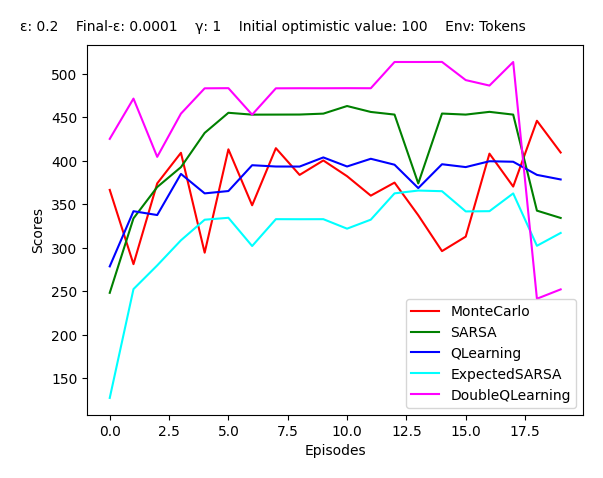
\includegraphics[width=0.7\textwidth]{tokensEnv}
    \caption{\texttt{Tokens} example}
    \label{fig:tokens}
\end{figure}

The Tokens environment is characterized by its simplicity, as it lacks obstacles that pose a lethal threat to the agent. The agent's task is to collect tokens at regular intervals to prevent its battery from draining completely. The number of rotations needed in this environment is six, making it relatively easy to train. Figure \ref{fig:tokens} illustrates that the average performance of all agents is commendable, even when \texttt{n=20}\footnote{Note that smoothing was applied to this plot.}. In subsequent sections, we will delve into more intriguing findings when tokens are incorporated into a larger environment, and explore their impact on the behaviour of the agents.

\section{Bugs and Viruses environment}
In this section, we aim to investigate two types of environments that have not been discussed before: Bugs and Viruses. These environments include three (\texttt{Worm, LadibugWalkingm LadybugFlying}) and two (\texttt{Bacteriophage, Rotavirus}) obstacles, respectively, and are different from environments that consist solely of trap-type obstacles. One key difference is that the agent can also use its ability to shoot in \texttt{Bugs} and \texttt{Viruses} environments. This means that, for the first time in this chapter, our agents have 6 actions to choose from, and we aim to analyse how this affects their behaviour.

\begin{figure}[h]
    \centering
    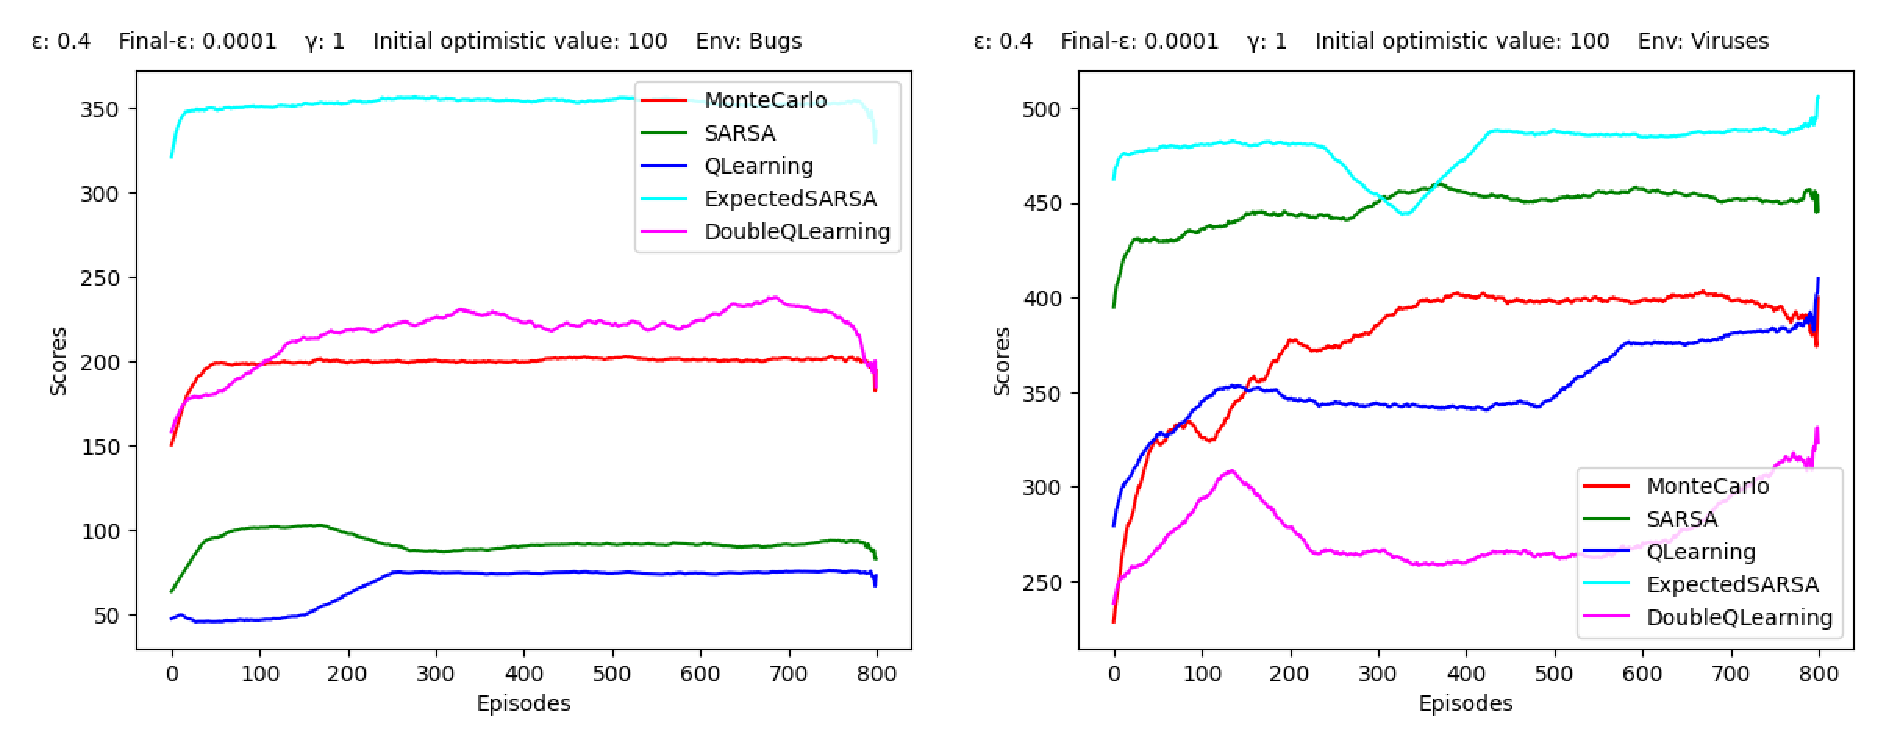
\includegraphics[width=\textwidth]{BV800ns}
    \caption{\texttt{Bugs} and \texttt{Viruses} environments examples}
    \label{fig:bv800ns_eg}
\end{figure}
\begin{figure}[h]
    \centering
    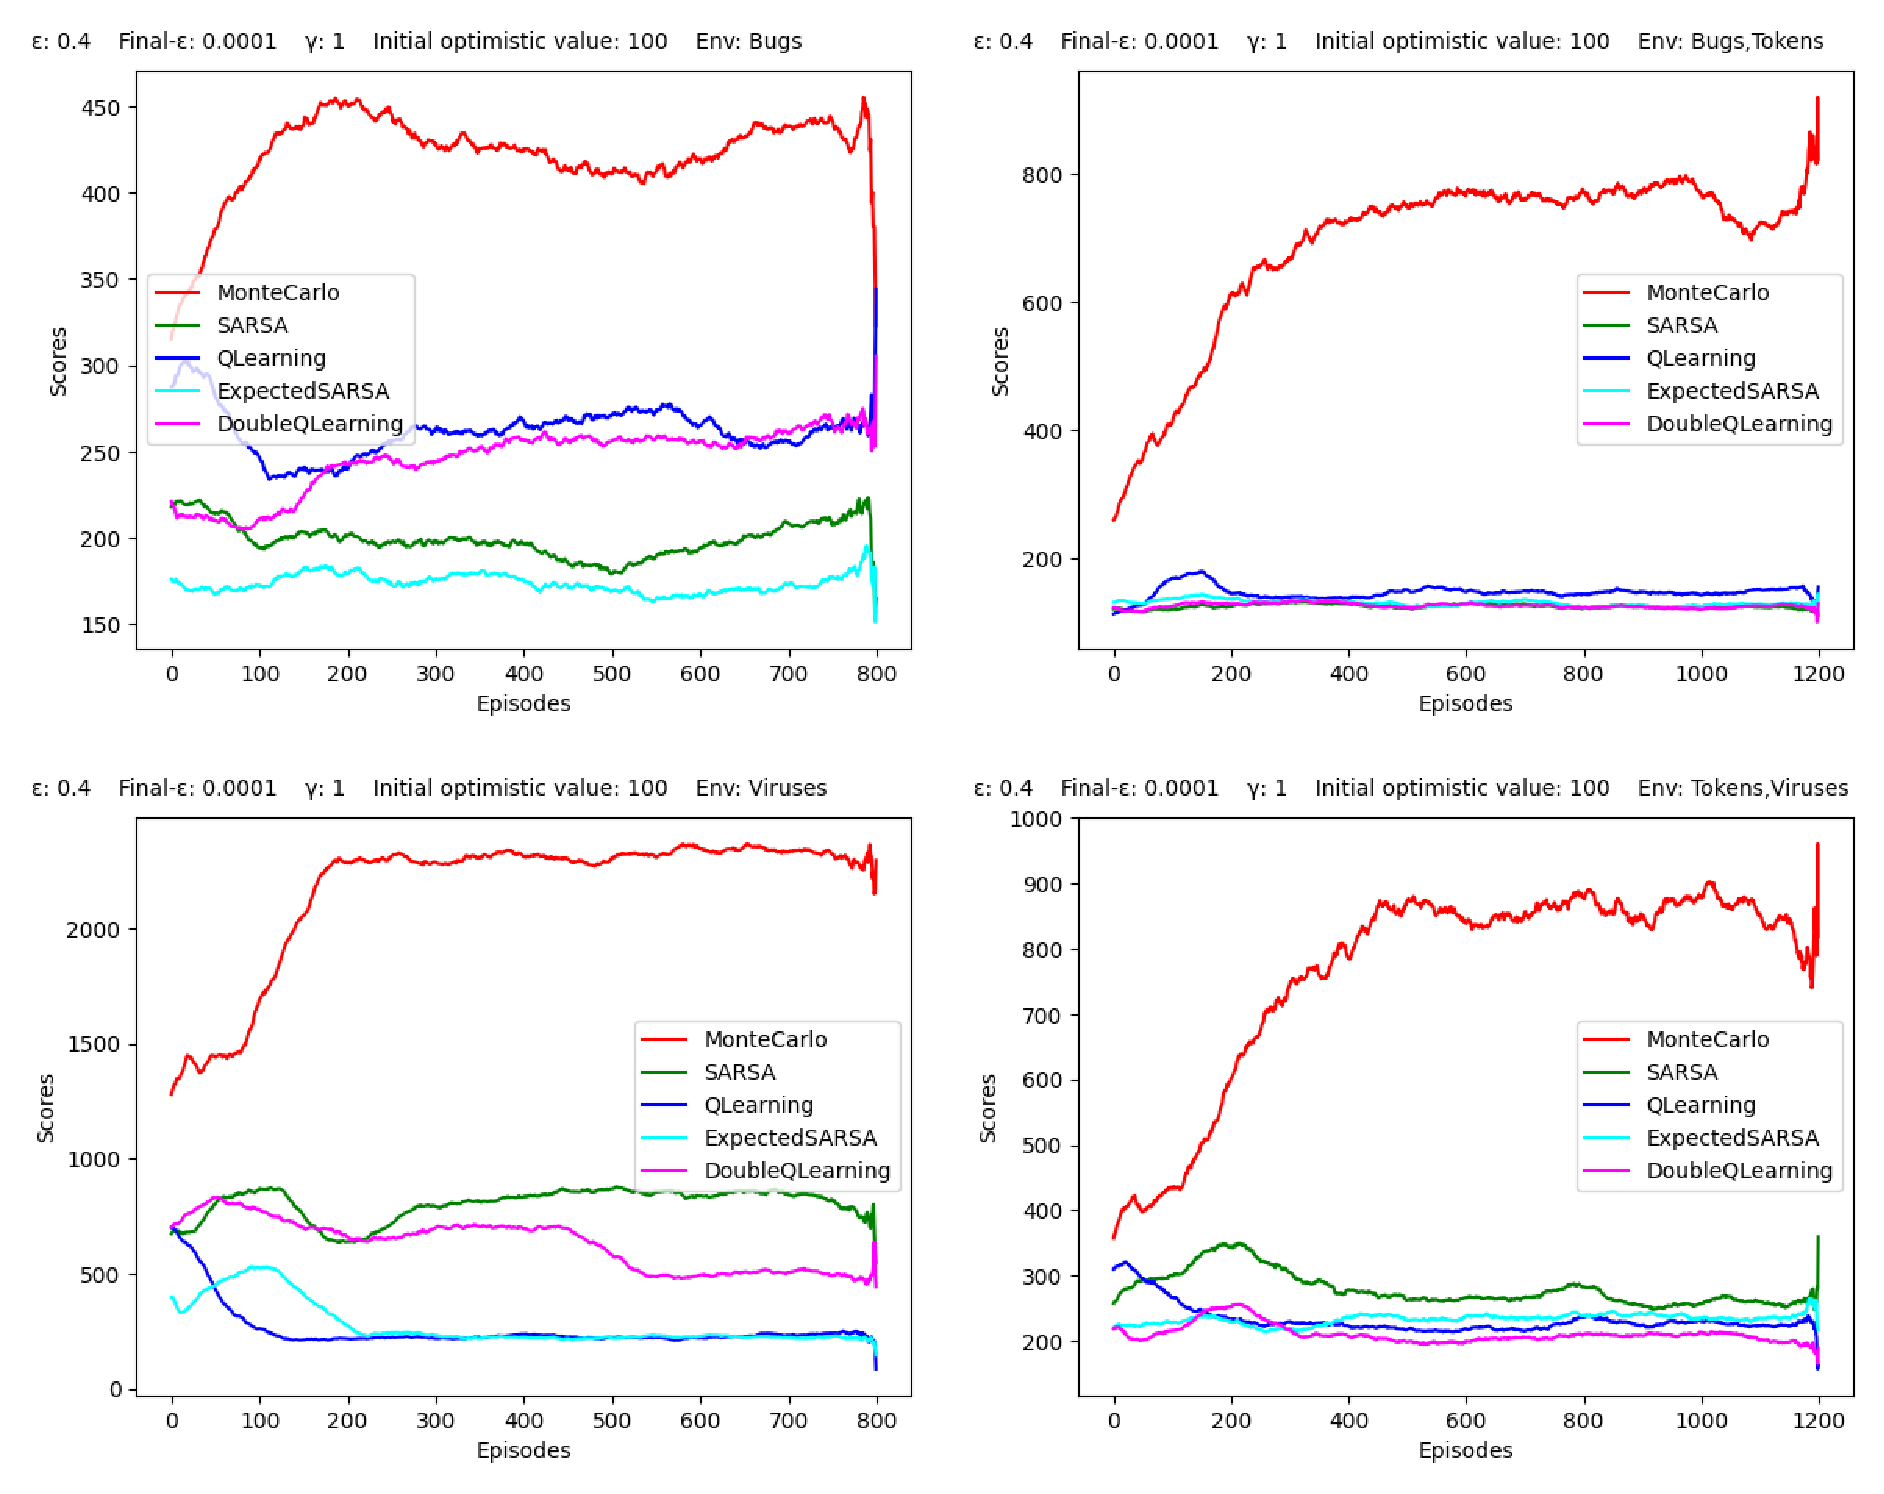
\includegraphics[width=\textwidth]{bbt_vvt}
    \caption{\texttt{Bugs},\texttt{Viruses} and their combination with \texttt{Tokens} examples}
    \label{fig:bbt_vvt_eg}
\end{figure}
\begin{figure}[h]
    \centering
    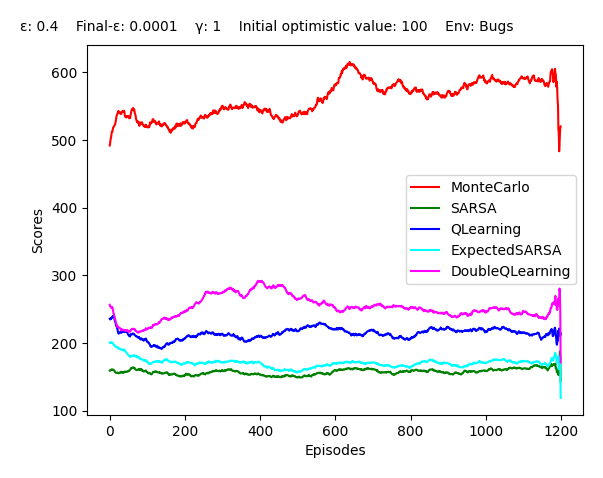
\includegraphics[width=0.7\textwidth]{bs_all_1200}
    \caption{\texttt{Bugs} with more games example}
    \label{fig:bs_all_120_eg}
\end{figure}
\begin{figure}[h]
    \centering
    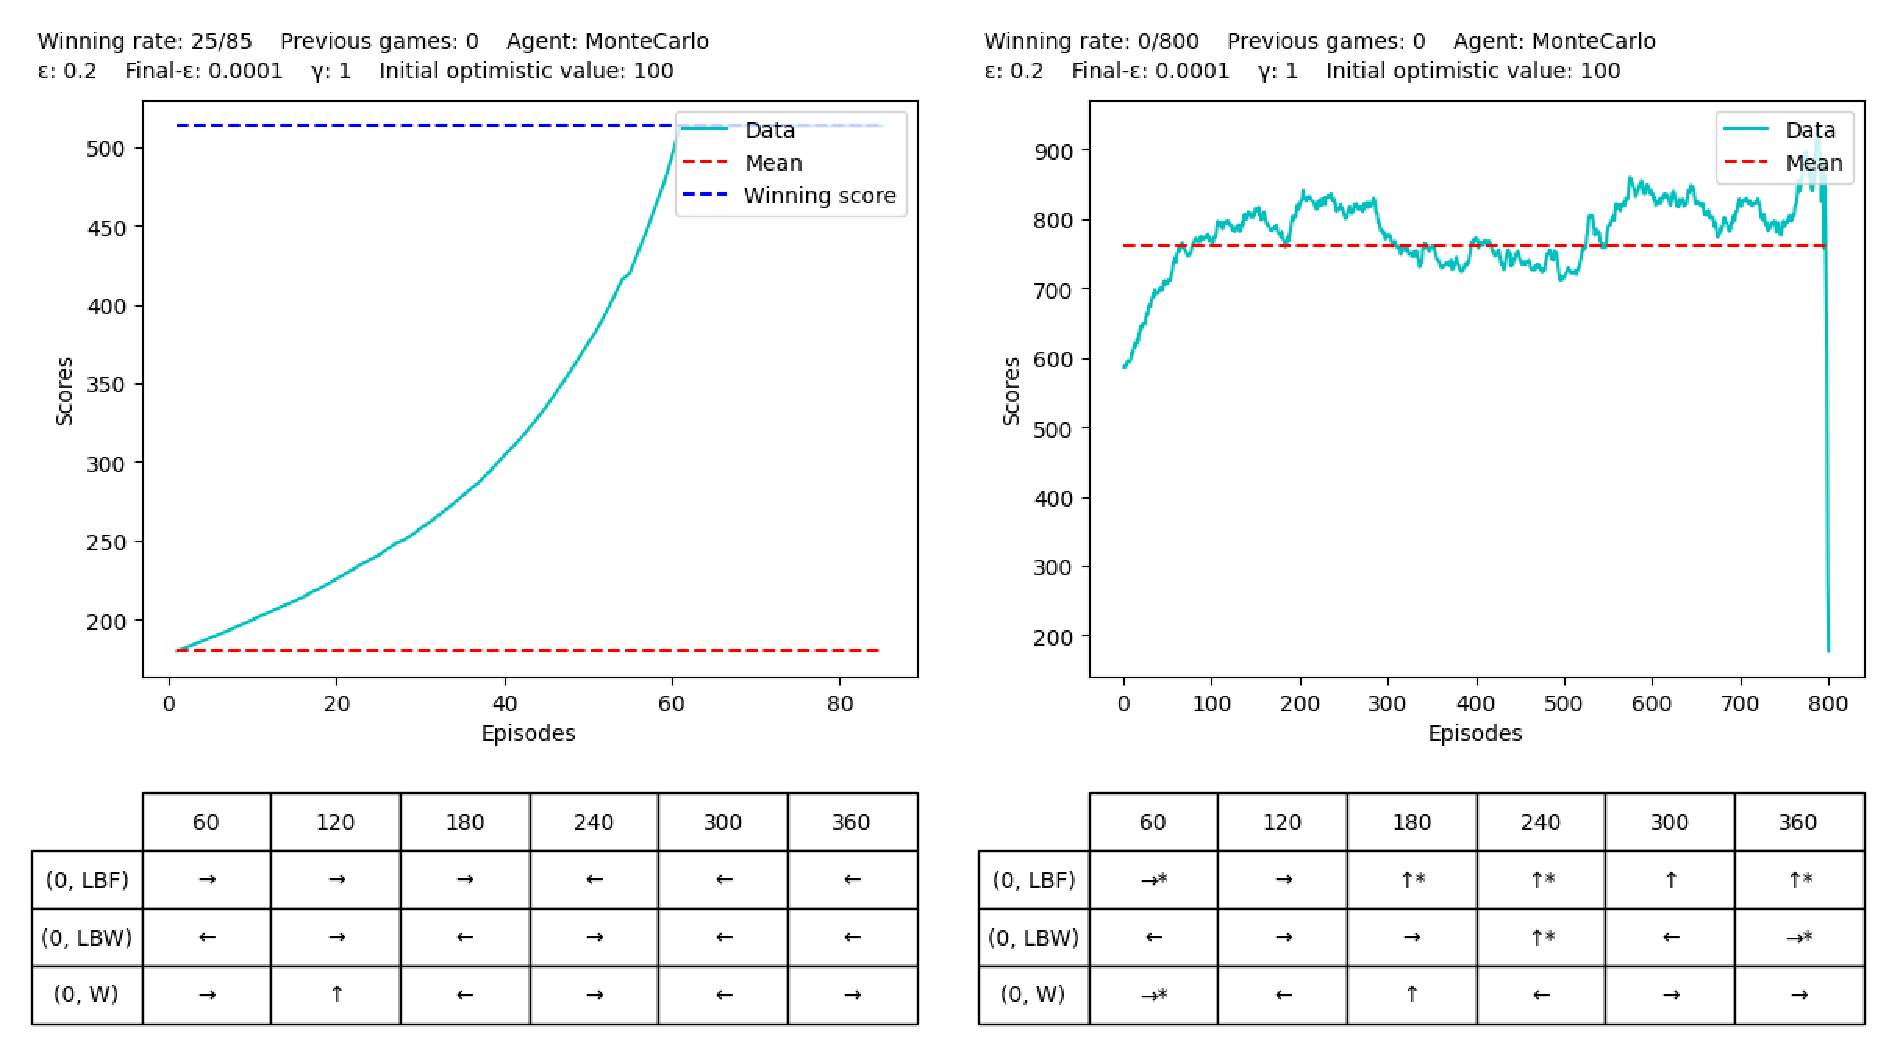
\includegraphics[width=\textwidth]{B_02_100_1}
    \caption{\texttt{Bugs} with and without shooting comparison}
    \label{fig:B_02_100_1_eg}
\end{figure}
\begin{figure}[h]
    \centering
    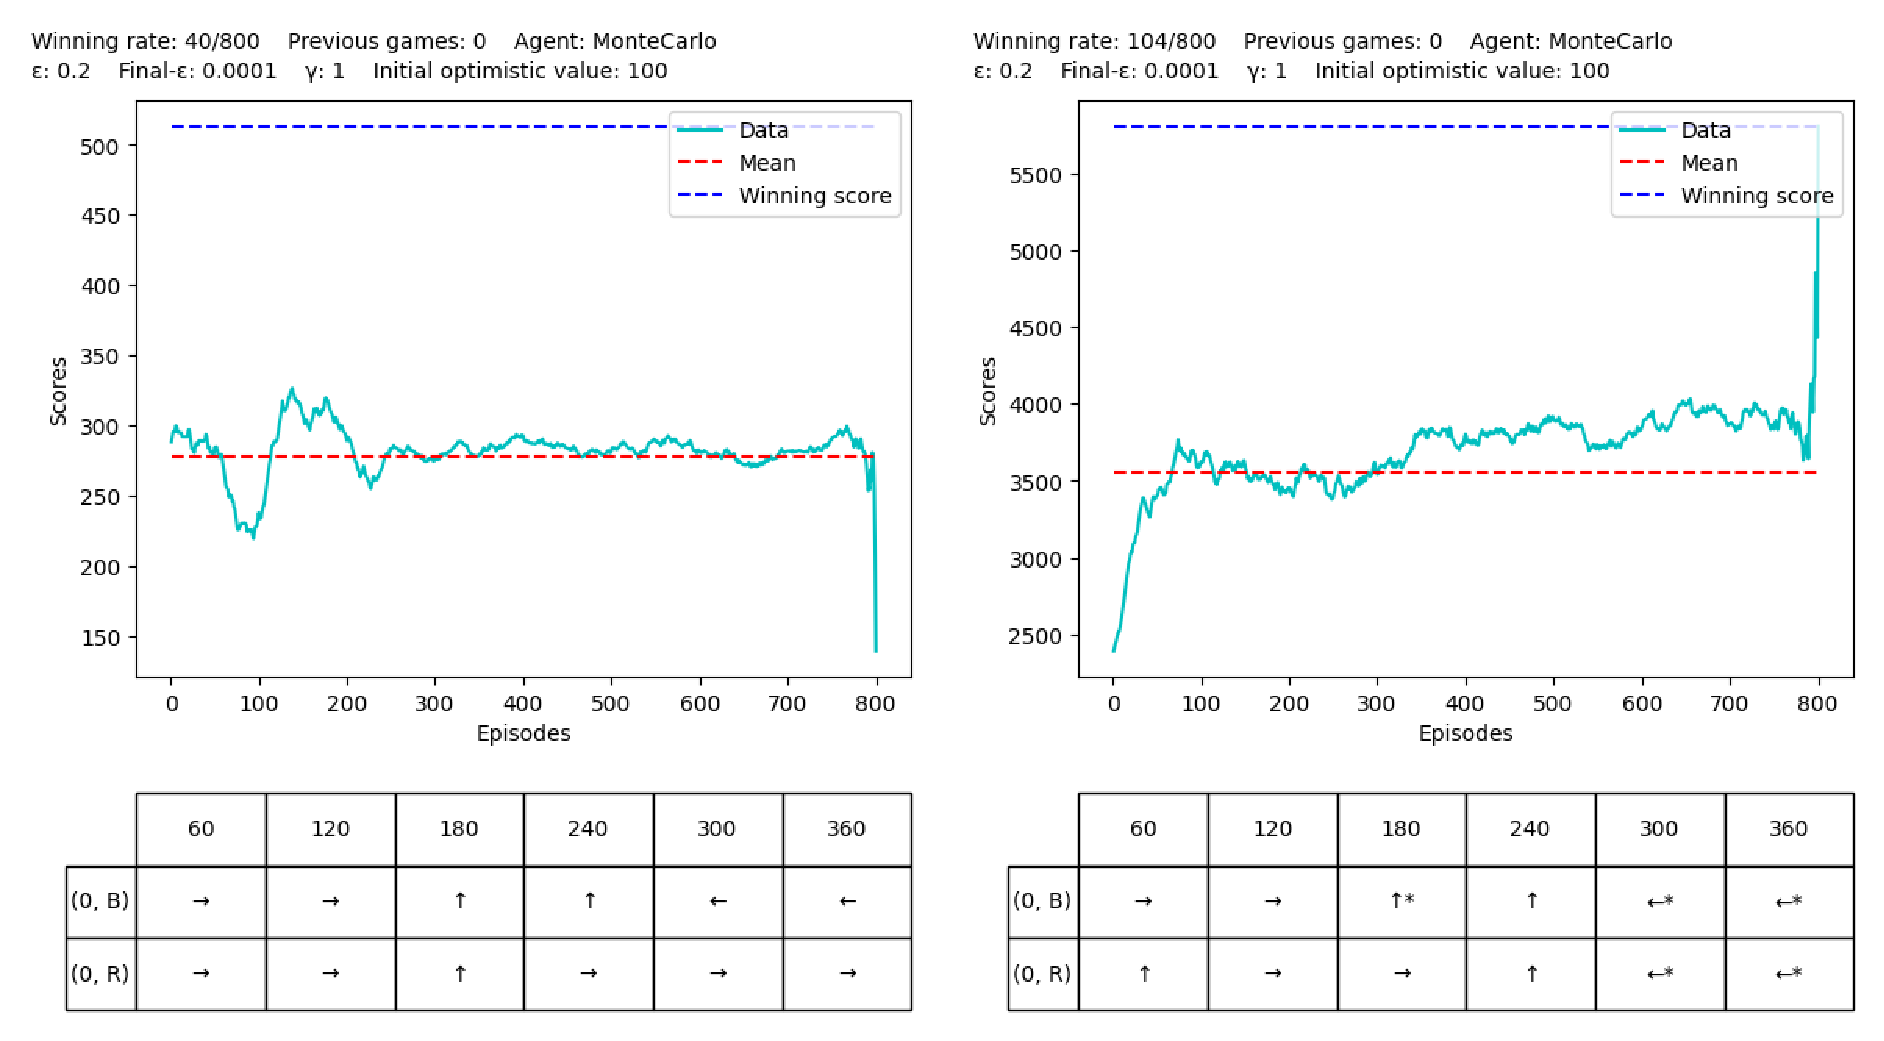
\includegraphics[width=\textwidth]{V_02_100_1}
    \caption{\texttt{Viruses} with and without shooting comparison}
    \label{fig:V_02_100_1_eg}
\end{figure}
\begin{figure}[h]
    \centering
    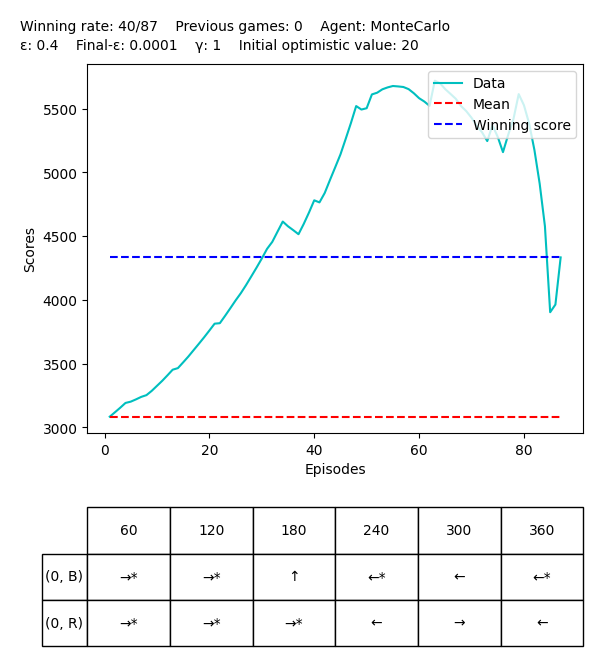
\includegraphics[width=0.7\textwidth]{viruses_interesting_s}
    \caption{Peculiar \texttt{Viruses} example}
    \label{fig:viruses_interesting_s_eg}
\end{figure}

\section{Full game environment}